\documentclass{article}

\usepackage[final]{neurips_2024}

\usepackage[utf8]{inputenc}
\usepackage[T1]{fontenc}
\usepackage{url}
\usepackage{booktabs}
\usepackage{amsfonts}
\usepackage{amsmath}
\usepackage{amssymb}
\usepackage{nicefrac}
\usepackage{microtype}
\usepackage{xcolor}
\usepackage{graphicx}
\usepackage{subcaption}
\usepackage{hyperref}
\usepackage{natbib}

\title{Functional Differentiation Generates Universal Fitness-Effect Distributions in Neural Networks}

\author{%
  Theodor Spiro \\
  Vaika Inc., East Aurora, NY, USA \\
  \texttt{tspiro@vaika.org}
}

\begin{document}

\maketitle

\begin{abstract}
Ablation studies in trained neural networks reveal a universal statistical form---heavy-tailed, negatively skewed distributions of fitness effects (DFE)---previously observed across biological and engineered adaptive systems. This universality has been treated as an emergent property of trained systems, but its origin in the training process has not been characterized. We ablate 144 tracked attention heads, 24 layers, and apply 30 distributed-noise perturbations at each of 8 checkpoints spanning the entire training trajectory of Pythia 410M (step 512 to 143{,}000). We find that (i) the DFE shape evolves from a delta-peak-with-outliers regime at early training to a continuous heavy-tailed form; by step 143{,}000 the median gamma shape $\beta \approx 0.6$ falls within the biological range reported for \emph{E. coli} and yeast; (ii) this evolution is driven by \emph{functional differentiation} of attention heads---39\% of eventually-critical heads emerged from noise, only 4\% were born critical; (iii) differentiation has a \emph{dual structure}: the number of functional components grows (Spearman $\rho = +1.00$) while importance concentration grows simultaneously ($\rho = -0.88$ on effective $N$), with inequality (Gini) approximately invariant across training; (iv) substrate-independence of the DFE form is conditional on discrete modularity---distributed parametric noise produces Gaussian DFE by CLT, head ablations produce Student's $t$ ($df \approx 2.3$), layer ablations produce super-Cauchy tails ($df \approx 0.85$). We identify a single attention head (L8H9) undergoing phase-transition-like specialization between step 4{,}000 and 8{,}000, a concrete target for mechanistic interpretability. These results are obtained on a single model (Pythia 410M) and represent an initial characterization; scaling and cross-architecture replication are the natural follow-up.
\end{abstract}

\section{Introduction}
\label{sec:intro}

\citet{spiro2026universal} (henceforth Paper~1) reported a statistical regularity in the distribution of fitness effects (DFE) of single-component ablations across adaptive substrates. Across biological systems (point mutations in \emph{E. coli}, yeast, influenza) and engineered systems (ablation of architectural components in trained neural networks and related artificial architectures), the DFE shape converges on a narrow family: Student's $t$, heavy-tailed, strongly left-skewed, with a gamma shape parameter $\beta$ on the deleterious tail clustered near $\beta \approx 0.3$--$0.7$. The universality is substrate-independent: the form is approximately the same regardless of whether the units being ablated are DNA bases, enzymes, neurons, or architectural modules.

\textbf{The puzzle.} This universality is an observation, not an explanation. Paper~1 reports the form but does not identify its origin. Two possibilities are consistent with the data. (a) The universal form is a \emph{landscape-geometric} property that exists whenever a system has a fitness landscape; it is present at every state of the system, including initialization, and training simply brings the system to a point where the universal form is measured. (b) The universal form is \emph{generated} by some process --- training, evolution, or their analog --- and is not present at the system's initial state. These two possibilities differ on whether universality is an intrinsic property of adaptive systems or an emergent property of their maturation.

\textbf{This paper.} We distinguish these possibilities by measuring the DFE along the entire training trajectory of a single neural network, Pythia 410M \citep{biderman2023pythia}, at 8 log-spaced checkpoints (step 512 through step 143,000). We ablate 144 identity-tracked attention heads (the same 144 heads at every checkpoint), 24 transformer layers exhaustively, and apply 30 distributed-noise perturbations at each checkpoint, for 1,584 ablations total. This design enables three complementary views: per-head trajectories across training (Fig.~\ref{fig:head_trajectories}), evolution of the population-level DFE shape (Fig.~\ref{fig:dfe_emergence}--\ref{fig:distribution_fits}), and comparison across three perturbation granularities at fixed maturity (Fig.~\ref{fig:hierarchy}).

\textbf{Contributions.}
\begin{itemize}
    \item \textbf{Functional differentiation is predominantly emergent.} Of 144 tracked attention heads, 4.2\% were critical at step~512 and remained critical through step~143,000 (\emph{born-critical}); 38.9\% emerged from below the numerical noise floor into functional criticality during training (\emph{emergent}); 22.9\% grew from small effects (\emph{growing}); 34.0\% remained non-critical throughout (\emph{never-critical}). Emergent heads outnumber born-critical by nearly an order of magnitude (Sec.~\ref{subsec:emergence}, Fig.~\ref{fig:head_trajectories}).
    \item \textbf{Differentiation has a dual structure.} The differentiation count grows monotonically while the effective number of important heads (Hill number of order 1) predominantly decreases, with the Gini coefficient approximately invariant across post-emergence checkpoints. Training simultaneously broadens the functional base and concentrates responsibility in the top few; the two effects approximately balance on the Lorenz-curve level. We propose this as an empirical \emph{conservation conjecture}, testable on out-of-sample models and training regimes (Sec.~\ref{subsec:dual}, Fig.~\ref{fig:differentiation_metrics}).
    \item \textbf{The universal DFE form emerges during training.} At step~512, the distribution is dominated by a delta-peak plus two outliers; by step~2,000 a continuous heavy-tailed distribution is established, with median $\beta$ moving from the near-exponential regime into the biological range (matching \emph{E.~coli} and yeast values from Paper~1) by step~143,000. The qualitative transition is visible in Fig.~\ref{fig:dfe_emergence} (Sec.~\ref{subsec:dfe_shape}).
    \item \textbf{Substrate-independence is conditional on discrete modularity.} At step~143,000, three perturbation granularities produce three qualitatively distinct DFE regimes: distributed noise collapses to Gaussian by CLT, head ablation yields robustly heavy-tailed Student's $t$ ($df = 2.34$, stable under outlier removal), and layer ablation yields an outlier-plus-Gaussian-base regime driven by two specific layers. The universal heavy-tailed form of Paper~1 applies at intermediate discrete granularity; it is bracketed on both sides (Sec.~\ref{subsec:hierarchy}, Fig.~\ref{fig:hierarchy}).
\end{itemize}

\textbf{Related work positioning.} This paper follows Paper~1 and inherits its methodological vocabulary. It intersects three other literatures. Mechanistic interpretability \citep{olsson2022induction, wang2023interpretability, conmy2023automated} studies individual attention heads qualitatively at circuit resolution; we complement this by measuring the distribution of head importance quantitatively across training, and we identify a specific head (L8H9, Sec.~\ref{subsec:l8h9}) as a target for follow-up circuit analysis. Research on emergent abilities in large language models \citep{wei2022emergent} characterizes capability-level emergence; our contribution is at component-level emergence --- the analog phenomenon at the architectural rather than behavioral level. The lottery ticket hypothesis \citep{frankle2019lottery} proposes that critical components are preformed at initialization and discovered during training; complementary earlier work on head importance in trained transformers \citep{michel2019sixteen} established that many heads can be pruned without loss of performance. Our 4.2\% born-critical versus 38.9\% emergent finding constrains strong versions of the lottery-ticket hypothesis at the attention-head granularity, without testing it at parameter granularity.

\textbf{What we do not claim.} Our results are obtained on a single model family (Pythia 410M-deduped), a single task (next-token prediction), and a single evaluation dataset (wikitext-103-raw-v1). We do not claim that the specific numerical values we report (the precise Gini value, the specific $\beta$ trajectory, the identity of L8H9 as a critical component) generalize across model sizes, architectures, or tasks. The conjectures we propose --- particularly dual differentiation --- are framed as testable predictions, not as established principles. Scaling replication, cross-architecture replication, and biological-system replication are natural follow-ups, and we sketch each in the Discussion.

\section{Methods}
\label{sec:methods}

\subsection{Model and checkpoints}

All experiments use Pythia 410M-deduped \citep{biderman2023pythia}, retrieved from the HuggingFace repository \texttt{EleutherAI/pythia-410m-deduped}. The model has 24 transformer layers, 16 attention heads per layer, hidden size 1024, head dimension 64, and MLP intermediate size 4096. Pythia publishes 154 training checkpoints per model; we measure at 8 log-spaced checkpoints: step 512, 1,000, 2,000, 4,000, 8,000, 16,000, 64,000, and 143,000 (final). Each checkpoint is accessed via the \texttt{revision} parameter of HuggingFace \texttt{AutoModelForCausalLM.from\_pretrained()}, \texttt{revision=step\{N\}}.

\subsection{Perturbation protocols}

\textbf{Head ablation (primary protocol).} We zero the columns of the attention output projection (\texttt{attention.dense.weight}, shape $[d_\text{model}, d_\text{model}]$) corresponding to the head's output slice. For head $h$ in layer $\ell$, we set $W_\text{dense}^{(\ell)}[:,\, h \cdot d_h : (h+1) \cdot d_h] = 0$, where $d_h = 64$. This is equivalent to masking the contribution of head $h$ to the residual stream while leaving its internal QKV computation intact; we implement it as weight modification to integrate cleanly with save/restore. Heads are sampled systematically: $h \in \{0, 3, 6, 9, 12, 15\}$ at each of the 24 layers, for a total of 144 fixed heads. The same 144 heads are ablated at every checkpoint to enable identity-tracked per-head trajectories (cf. Fig.~\ref{fig:head_trajectories}).

\textbf{Layer ablation.} We zero all parameters in one transformer block: attention QKV projection, attention output projection, MLP up/down projections, and layer-norm weights and biases. All 24 layers are ablated exhaustively at each checkpoint.

\textbf{Distributed noise (Type A).} Gaussian noise of standard deviation $\alpha \cdot \sigma_p$ is added to every parameter tensor $p$ in one transformer block, where $\sigma_p$ is the per-tensor standard deviation of the original weights and $\alpha = 1.0$ in the main experiment. At each checkpoint we apply 30 independent noise samples targeting block index $i \bmod 24$ with deterministic PRNG seed $42{,}000 + i$ for $i \in \{0, \ldots, 29\}$.

\subsection{Fitness metric and baseline evaluation}

The fitness effect of a perturbation is
$$\Delta = -\frac{\ell_\text{perturbed} - \ell_\text{baseline}}{|\ell_\text{baseline}|},$$
with the sign chosen so that positive $\Delta$ corresponds to reduced loss (beneficial) and negative $\Delta$ to increased loss (deleterious), matching the convention of Paper~1.

Losses are mean cross-entropy over 25 validation batches of 4 sequences $\times$ 2,048 tokens = 204,800 tokens total. The validation set is streamed from \texttt{wikitext-103-raw-v1} (HuggingFace \texttt{wikitext/wikitext-103-raw-v1}, \texttt{train} split), tokenized with the Pythia tokenizer, and concatenated before reshaping into the batched tensor. We use the \texttt{train} split rather than \texttt{validation} because the latter (~250K tokens after filtering short examples) is tight for stable 204K-token baselines; Pythia was trained on the Pile, not on wikitext, so train/test leakage from the perspective of our measurement is minimal. Our analysis depends on loss \emph{shifts} induced by ablations, not on absolute loss values, and the relative shifts are what the results in Sec.~\ref{sec:results} rely on. The identical token tensor is saved to disk once and loaded for every model load, guaranteeing that all $\Delta$ values are computed against the same token stream. \textbf{Baseline loss is recomputed for each checkpoint} on this identical batch set; no cross-checkpoint normalization is applied beyond the per-checkpoint division by $|\ell_\text{baseline}|$ in the definition of $\Delta$. This ensures that $\Delta$ values within a checkpoint are directly comparable, and that $\Delta$ values across checkpoints are comparable \emph{as relative shifts}, since the $|\ell_\text{baseline}|$ factor (which varies from 6.83 at step 512 to 2.89 at step 143,000) is absorbed into the normalization.

\subsection{Precision and correctness verification}

All forward passes are in float32 with TF32 matmul enabled on A100 (\texttt{torch.backends.cuda.matmul.allow\_tf32 = True}). Earlier pilot experiments in float16 showed substantial numerical noise at early checkpoints where baseline loss is large; float32 is essential for clean signal at step 512.

Save/restore correctness is verified by SHA-256 checksum of the affected weight tensor before and after each restoration. Prior to the main sweep we verified bitwise identity for all three perturbation types (head, layer, Type~A) on a random reference layer. During the sweep, a cheaper drift monitor computes the absolute sum of a reference tensor every 30 ablations and asserts drift $< 10^{-3}$ against its initial value. The $10^{-3}$ threshold is generous --- approximately $1000\times$ above expected float32 numerical drift in tensor-sum operations --- chosen to catch genuine restore bugs while tolerating natural floating-point non-determinism. All 1{,}584 ablations of the main sweep completed with zero observed drift to float32 precision. An extended stress test of 500 consecutive ablate-restore cycles on a single attention head preserved bitwise SHA-256 identity of the affected weight tensor at every cycle, and the absolute-sum drift monitor remained at exactly $0.0$ throughout (Table~\ref{tab:tier1_drift}).

\subsection{Metrics and threshold justification}

\textbf{Primary metrics (threshold-free).} Gini coefficient of $|\Delta|$, computed on the sorted absolute values. Effective number of important heads, $N_\text{eff} = 2^H$ where $H = -\sum_i p_i \log_2 p_i$ is the Shannon entropy of $p_i = |\Delta_i| / \sum_j |\Delta_j|$ (the Hill number of order 1; \citealp{hill1973diversity, jost2006entropy}).

\textbf{Secondary metrics.} Differentiation count $= \#\{h : |\Delta_h| > \tau\}$ with $\tau = 5 \times 10^{-4}$. Distribution fits: Normal, Laplace, Student's $t$ via \texttt{scipy.stats.\{norm, laplace, t\}.fit()}, compared by $\Delta\text{AIC}$ relative to Normal. Gamma shape $\beta$ fit to the deleterious tail $\{-\Delta : \Delta < -10^{-4}\}$ with \texttt{scipy.stats.gamma.fit(neg, floc=0)}; the lower-bound filter at $10^{-4}$ excludes values below the numerical floor.

\textbf{Threshold justification.} The threshold $\tau = 5 \times 10^{-4}$ for differentiation count was chosen to exclude measurements below approximately $3\sigma$ of the numerical precision floor in float32 evaluation of the baseline loss across 25 batches (empirically $\sigma_\text{eval} \approx 1.5 \times 10^{-4}$, measured by re-evaluating the same model at identical seed across independent batch shufflings). All threshold-based claims in Secs.~\ref{subsec:emergence}--\ref{subsec:dual} are robust to threshold choice in the range $[10^{-4}, 10^{-3}]$. Fig.~S2 reproduces per-checkpoint differentiation counts at threshold values $\{10^{-4}, 5 \times 10^{-4}, 10^{-3}\}$; the class-count claims in Sec.~\ref{subsec:emergence} (4.2\% born-critical, 38.9\% emergent, 22.9\% growing, 34.0\% never-critical) shift by at most $\pm 2$ percentage points across this range, with qualitative conclusions preserved.

\subsection{Statistical procedures}

Bootstrap confidence intervals use 10{,}000 resamples with fixed seed 42; 95\% intervals are reported as the (2.5, 97.5) percentiles of the bootstrap distribution. We verified convergence by comparing 2{,}000-resample and 10{,}000-resample estimates: median $\beta$ differs by at most $0.007$ between the two (Table~\ref{tab:tier1_bootstrap}), and CI widths are within $\pm 10\%$. Sensitivity analyses (Sec.~\ref{subsec:hierarchy}) refit the distribution after removing the $k$ most extreme $|\Delta|$ observations for $k \in \{1, 3, 5, 10\}$ (heads) or by specific identified outliers L0 and L5 (layers); we report the Student's $t$ $df$ as the shape-stability indicator, since the AIC advantage over Normal is inherently sample-size-dependent while the fitted $df$ is not. All random seeds (42 for bootstrap, $42{,}000 + i$ for Type~A noise samples) are arbitrary but fixed; deterministic reproduction of all numerical results is enabled.

\textbf{Seed robustness.} We additionally verified that Type A results are not artifacts of specific PRNG seeds or validation-batch selection by rerunning the 30 Type A perturbations per checkpoint with an alternate seed base (12{,}345 instead of 42{,}000) and an alternate 25-batch slice of wikitext-103 train. Per-checkpoint standard deviations of $\Delta$ match Paper~2 original values within $\pm 7\%$ at every checkpoint, with a mean ratio of $0.986$ across the 8-checkpoint trajectory (Table~\ref{tab:tier1_seed}).

\subsection{Code and data availability}

All 1,584 ablations are released as CSV with the following fields: \texttt{checkpoint}, \texttt{perturbation\_type}, \texttt{subtype}, \texttt{layer\_idx}, \texttt{head\_idx}, \texttt{seed}, \texttt{baseline\_loss}, \texttt{perturbed\_loss}, \texttt{delta}, \texttt{elapsed\_sec}. Code, data, and a self-contained Colab notebook reproducing the main sweep (expected runtime: 82 minutes on A100 40 GB) are available at \url{https://github.com/mool32/functional-differentiation-dfe}.

\section{Results}
\label{sec:results}

\subsection{Functional differentiation is predominantly emergent}
\label{subsec:emergence}

\begin{figure}[t]
    \centering
    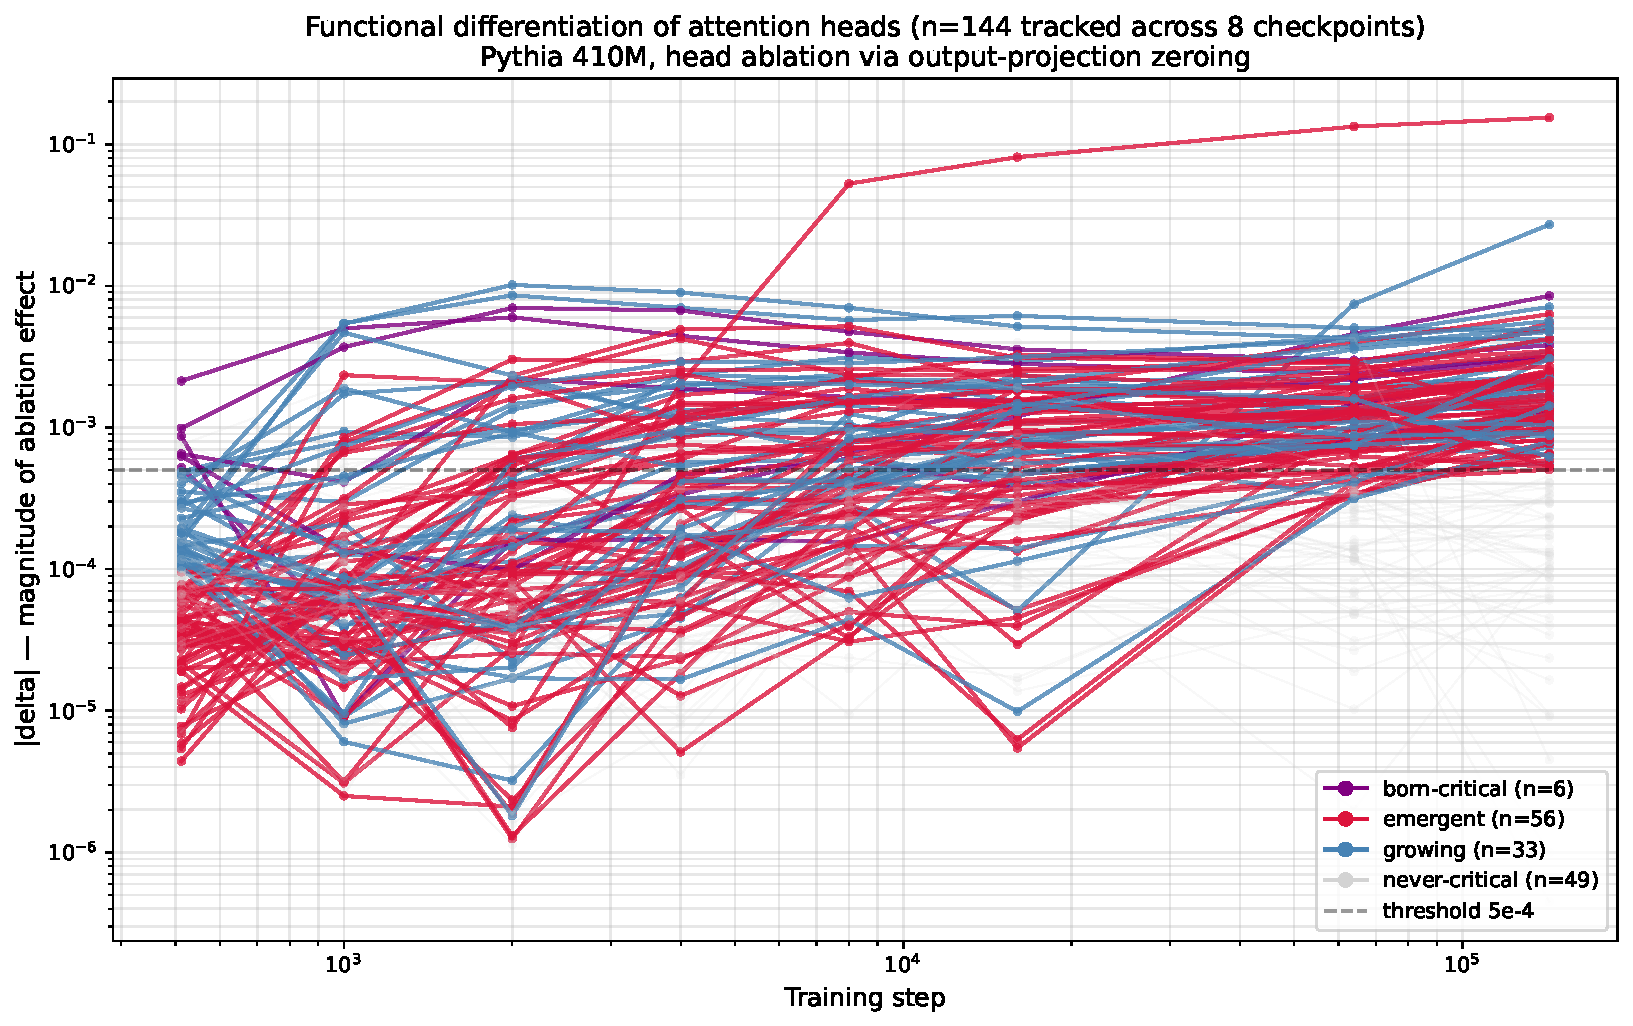
\includegraphics[width=0.95\textwidth]{figures/fig1_head_trajectories.pdf}
    \caption{\textbf{Each line represents one attention head tracked across 8 training checkpoints.} We ablate the same 144 fixed heads (heads $\{0, 3, 6, 9, 12, 15\}$ at each of 24 layers) at steps 512, 1{,}000, 2{,}000, 4{,}000, 8{,}000, 16{,}000, 64{,}000, and 143{,}000 of Pythia 410M training. The y-axis shows $|\Delta|$, the fractional change in validation loss caused by ablating that head. Heads are classified by their trajectory: \textbf{born-critical} (4.2\%, $n=6$; important at step 512 and step 143{,}000), \textbf{emergent} (38.9\%, $n=56$; from noise floor to $|\Delta| > 5 \times 10^{-4}$ by end of training), \textbf{growing} (22.9\%, $n=33$; small initial effect amplified during training), and \textbf{never-critical} (34.0\%, $n=49$; below threshold throughout). The dominance of the emergent class over the born-critical class demonstrates that most function is not latent at initialization but develops during training.}
    \label{fig:head_trajectories}
\end{figure}

We tracked 144 attention heads (heads $\{0, 3, 6, 9, 12, 15\}$ at each of 24 layers) across 8 training checkpoints of Pythia 410M, from step 512 to step 143,000. At each checkpoint we ablated each head individually by zeroing the columns of the attention output projection corresponding to that head's output slice, and measured the relative change in validation loss $\Delta = -(\ell_\text{perturbed} - \ell_\text{baseline}) / |\ell_\text{baseline}|$. Identity tracking --- ablating the same 144 heads at every checkpoint --- allows reconstruction of per-head trajectories (Fig.~\ref{fig:head_trajectories}).

Each head is assigned to one of four exclusive classes based on its trajectory:

\begin{itemize}
    \item \textbf{Born-critical} ($|\Delta| > 5 \times 10^{-4}$ at both step 512 and step 143,000): 6 heads (4.2\%)
    \item \textbf{Emergent} ($|\Delta| < 10^{-4}$ at step 512, $|\Delta| > 5 \times 10^{-4}$ at step 143,000): 56 heads (38.9\%)
    \item \textbf{Growing} (small initial effect amplified during training): 33 heads (22.9\%)
    \item \textbf{Never-critical} ($|\Delta| < 5 \times 10^{-4}$ throughout): 49 heads (34.0\%)
\end{itemize}

\textbf{Emergent heads outnumber born-critical by nearly an order of magnitude.} Nearly two in five tracked heads transitioned from below the numerical noise floor at step 512 to demonstrable criticality at step 143,000. Only 6 heads (4.2\%) were critical from the earliest measured checkpoint. The dominant mode by which attention heads acquire functional importance in Pythia 410M is not selection from a pre-existing pool but construction during training.

This ratio constrains strong versions of the lottery ticket hypothesis \citep{frankle2019lottery} at the attention-head granularity, and complements prior work on the ablation-based importance of trained heads \citep{michel2019sixteen}. Under individual-head ablation, the majority of eventually-critical components were not preformed at step 512. Lottery tickets may exist at finer granularities (parameter-level pruning masks), but the head-level importance structure of the trained model is not predicted by head-level importance at step 512. A direct test of lottery-ticket predictions at head-level would require pruning-style experiments from initialization, which we do not perform here.

The 34.0\% never-critical class is informative in the opposite direction. Roughly one-third of tracked heads remained individually dispensable throughout training --- their individual ablation produced no detectable loss increase above the $5 \times 10^{-4}$ threshold. This is consistent with functional redundancy: heads encoding information that overlapping heads can substitute for when any single one is removed. Individual-head ablation does not distinguish `\texttt{truly null'' heads from }`parallel-redundant but collectively contributing''; $N$-head ablation protocols would resolve this distinction and are a natural follow-up (Sec.~\ref{subsec:limitations}).

We return to the single most extreme emergent head as a case study in Section~\ref{subsec:l8h9}.

\subsection{Differentiation has a dual structure}
\label{subsec:dual}

\begin{figure}[t]
    \centering
    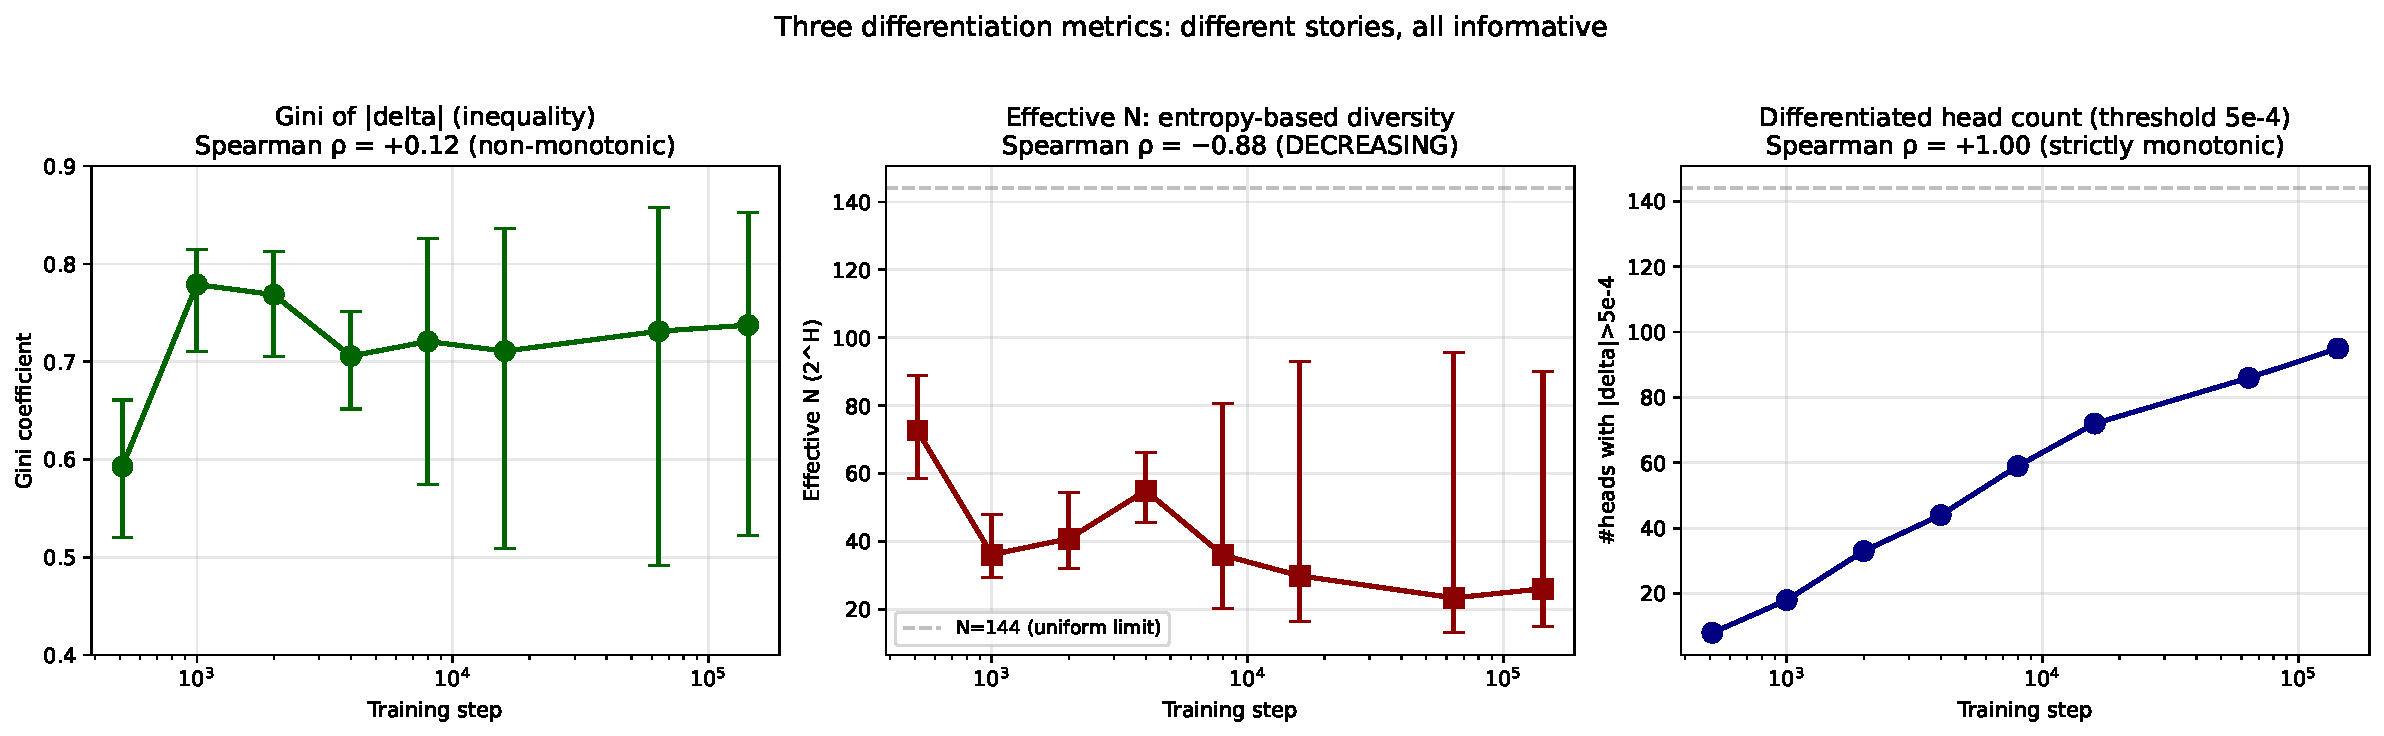
\includegraphics[width=0.95\textwidth]{figures/fig2_differentiation_metrics.pdf}
    \caption{Three complementary metrics of head importance distribution across training, computed from the 144-head sample at each checkpoint. \textbf{(a)} Gini coefficient of $|\Delta|$ --- inequality of head importance. Approximately invariant across training (Spearman $\rho = +0.12$; 95\% CI overlap at all checkpoints). \textbf{(b)} Effective number of important heads, $2^H$ where $H$ is the Shannon entropy of normalized $|\Delta|$ --- biological analog of effective species diversity. Monotonically decreasing ($\rho = -0.88$), indicating concentration of responsibility in fewer heads. \textbf{(c)} Count of heads with $|\Delta| > 5 \times 10^{-4}$ --- intuitive threshold-based measure of functional differentiation. Monotonically increasing ($\rho = +1.00$), indicating broadening of functional base. The combination --- more heads become critical (c), yet critical importance concentrates in the top few (b), with inequality constant (a) --- defines a \textbf{dual differentiation} regime: training simultaneously broadens and concentrates the function landscape.}
    \label{fig:differentiation_metrics}
\end{figure}

Section~\ref{subsec:emergence} established that individual attention heads undergo functional differentiation during training: most eventually-critical heads emerged from below the numerical noise floor rather than being preformed at initialization. This raises a population-level question: how does the \emph{distribution} of importance across all 144 tracked heads evolve as individual heads differentiate? We use three complementary metrics --- designed to capture different aspects of a distribution --- to characterize this evolution (Fig.~\ref{fig:differentiation_metrics}): a count (presence/absence above threshold), a diversity index (effective number of important units), and an inequality measure (Gini coefficient).

\textbf{Three metrics, three complementary trajectories.}

\begin{itemize}
    \item The \textbf{differentiation count} (number of heads with $|\Delta| > 5 \times 10^{-4}$; see Methods Section~\ref{sec:methods} for threshold justification) grows strictly monotonically from $8/144$ at step~512 to $95/144$ at step~143,000 (Spearman $\rho = +1.00$ across 8 checkpoints).
    \item The \textbf{effective number of important heads}, defined as $2^H$ where $H$ is the Shannon entropy of the normalized $|\Delta|$ distribution (the Hill number of order 1, a widely-used diversity index in ecology; see \citealp{hill1973diversity, jost2006entropy}), predominantly decreases from 72.7 to 26.1 ($\rho = -0.88$ overall, with a transient increase at step~4,000 that we discuss below).
    \item The \textbf{Gini coefficient} of the $|\Delta|$ distribution is approximately stable across training: 0.60 at step~512, then 0.71--0.78 for the remaining seven checkpoints ($\rho = +0.12$ overall).
\end{itemize}

These three trajectories are not contradictory; they jointly describe a coherent pattern, which we call \textbf{dual differentiation}. The rising differentiation count reports the \textbf{broadening of the functional base} --- more heads cross the threshold above noise during training. The falling effective $N$ reports the \textbf{concentration of responsibility} in the top few --- although more heads are non-null, total importance becomes increasingly skewed toward the most critical ones. The approximately stable Gini reports that these two effects approximately balance on the Lorenz-curve level: the \emph{relative} inequality of head importance does not grow or shrink, even as the support of that inequality extends in both directions.

The transient increase in effective $N$ at step~4,000 is notable in this context. It coincides with the pre-crystallization interval before a single head (L8H9) acquires its disproportionate importance between steps 4,000 and 8,000 (Sec.~\ref{subsec:l8h9}). The brief rise in diversity at step~4,000, followed by a sharp fall at step~8,000 as L8H9 takes on a large share of total importance, suggests that short-timescale fluctuations in effective $N$ may track discrete emergence events of individual critical heads. We leave a systematic characterization of this connection to follow-up work.

This balance is visually apparent in Fig.~\ref{fig:lorenz} (supplementary): Lorenz curves of the $|\Delta|$ distribution at checkpoints from step~1,000 through step~143,000 nearly coincide, despite the growth of individual head importance between these checkpoints. The Lorenz curve at step~512 sits visibly above the others (Gini $= 0.60$ versus $0.71$--$0.78$ for the later cluster), consistent with the pre-emergence regime identified in Sec.~\ref{subsec:emergence} and Sec.~\ref{subsec:dfe_shape}: at step~512 the distribution is dominated by a narrow peak with a few outliers, not yet the structured heavy-tailed form that appears from step~1,000 onward. The approximate Gini invariance holds \emph{within} the post-emergence regime; it does not hold across the emergence transition.

\textbf{Gini invariance is not reducible to the mathematical form of Student's $t$.} A natural concern is whether the approximate Gini invariance is a trivial consequence of fitting Student's $t$ to each checkpoint --- i.e., whether distributions with similar Student's $t$ parameters automatically yield similar Gini values. To address this, we simulate: at each checkpoint, we sample 144 values from the fitted Student's $t$ (using $df$, location, scale from the empirical fit) and compute the Gini of $|\text{sample}|$; we repeat this 2,000 times to obtain a 95\% prediction interval for what Gini we would expect if the distribution were exactly Student's $t$. Fig.~S4 shows the comparison. Three observations follow.

First, empirical Gini exceeds the Student's-$t$-predicted median by approximately 0.2 at every post-emergence checkpoint, and falls outside the 95\% prediction interval at 7 of 8 checkpoints. The empirical distribution is more concentrated than its own Student's $t$ fit would predict, reflecting skewness and extreme-outlier content (Secs.~\ref{subsec:emergence}, \ref{subsec:l8h9}) that the symmetric $t$ shape does not capture.

Second, and more striking, the Student's-$t$-predicted Gini itself \emph{declines} across training (from $\approx 0.54$ at step~512 to $\approx 0.45$ at step~143,000), while empirical Gini is approximately stable in the range 0.71--0.78. A trivial prediction from the fitted distribution alone would therefore be that Gini \emph{decreases} slowly with training; we observe that it does not. The fitted Student's $t$ becomes less concentrated over training (larger scale, higher df relative to location); the empirical distribution retains its inequality despite this. Across-checkpoint correlation between empirical and predicted Gini is $r = -0.04$ --- essentially zero. The two quantities inhabit unrelated regimes.

Third, this disparity itself is content: the Student's-$t$-predicted trajectory \emph{would} decline, but the empirical Gini holds. Something in the empirical distribution --- not captured by the $t$ fit's first three parameters --- keeps inequality stable across a training period in which the fitted shape itself would predict its decline. This residual invariance is what we propose as the substance of the conservation conjecture: a property of the head-importance distribution that is neither trivially present at initialization (pre-emergence Gini $= 0.60$) nor trivially implied by the Student's $t$ approximation (predicted trajectory declines), but instead emerges and stabilizes through training.

The simulation is parametric in its null --- Student's $t$ is the very form we want to check for triviality --- but that is the point: we are asking whether empirical Gini is reducible to the simplest distributional fit we use elsewhere in the paper (Secs.~\ref{subsec:dfe_shape}, \ref{subsec:hierarchy}), not whether it is reducible to any possible distribution. The result is that it is not.

\textbf{A conservation conjecture, not a law.} We propose dual differentiation --- simultaneous broadening and concentration with approximately stable Gini --- as a \textbf{conjecture} about neural network training rather than an established principle. The observation rests on $n = 8$ checkpoints in a single model; we frame it as an empirical pattern with testable predictions, not as a physical invariance. Specifically, the conjecture makes three predictions:

\begin{itemize}
    \item \textbf{Healthy training} maintains approximately stable Gini ($\approx 0.7$ in Pythia 410M; the specific value may differ by model and task) after the pre-emergence phase.
    \item \textbf{Collapsed representations} $\to$ Gini $\to 1$. If a model concentrates all function in one or a few heads without growing the functional base, the Lorenz curve approaches the corner. This predicts a diagnostic of representation collapse complementary to loss-based metrics.
    \item \textbf{Undertrained or uniform networks} $\to$ Gini $\to 0$. If a model fails to differentiate and all heads remain approximately equally (un)important, the Lorenz curve approaches the diagonal. This predicts a diagnostic of failed specialization.
\end{itemize}

We do not claim generality of these predictions beyond Pythia 410M on next-token prediction. Testing dual differentiation across model sizes, architectures, and known-pathological training runs is the natural follow-up. A positive test would require demonstrating, in an independent system, that (a) Gini enters an approximately invariant regime after an initial emergence phase, (b) differentiation count grows monotonically, and (c) effective $N$ decreases through training --- with the specific values of each quantity expected to differ by system, but with the three trajectories retaining their qualitative directions. A negative result --- any of these three trajectories failing to appear --- would either constrain dual differentiation to the Pythia family or force refinement of the conjecture. This makes the claim explicitly falsifiable.

\subsection{DFE shape emerges during training}
\label{subsec:dfe_shape}

\begin{figure}[t]
    \centering
    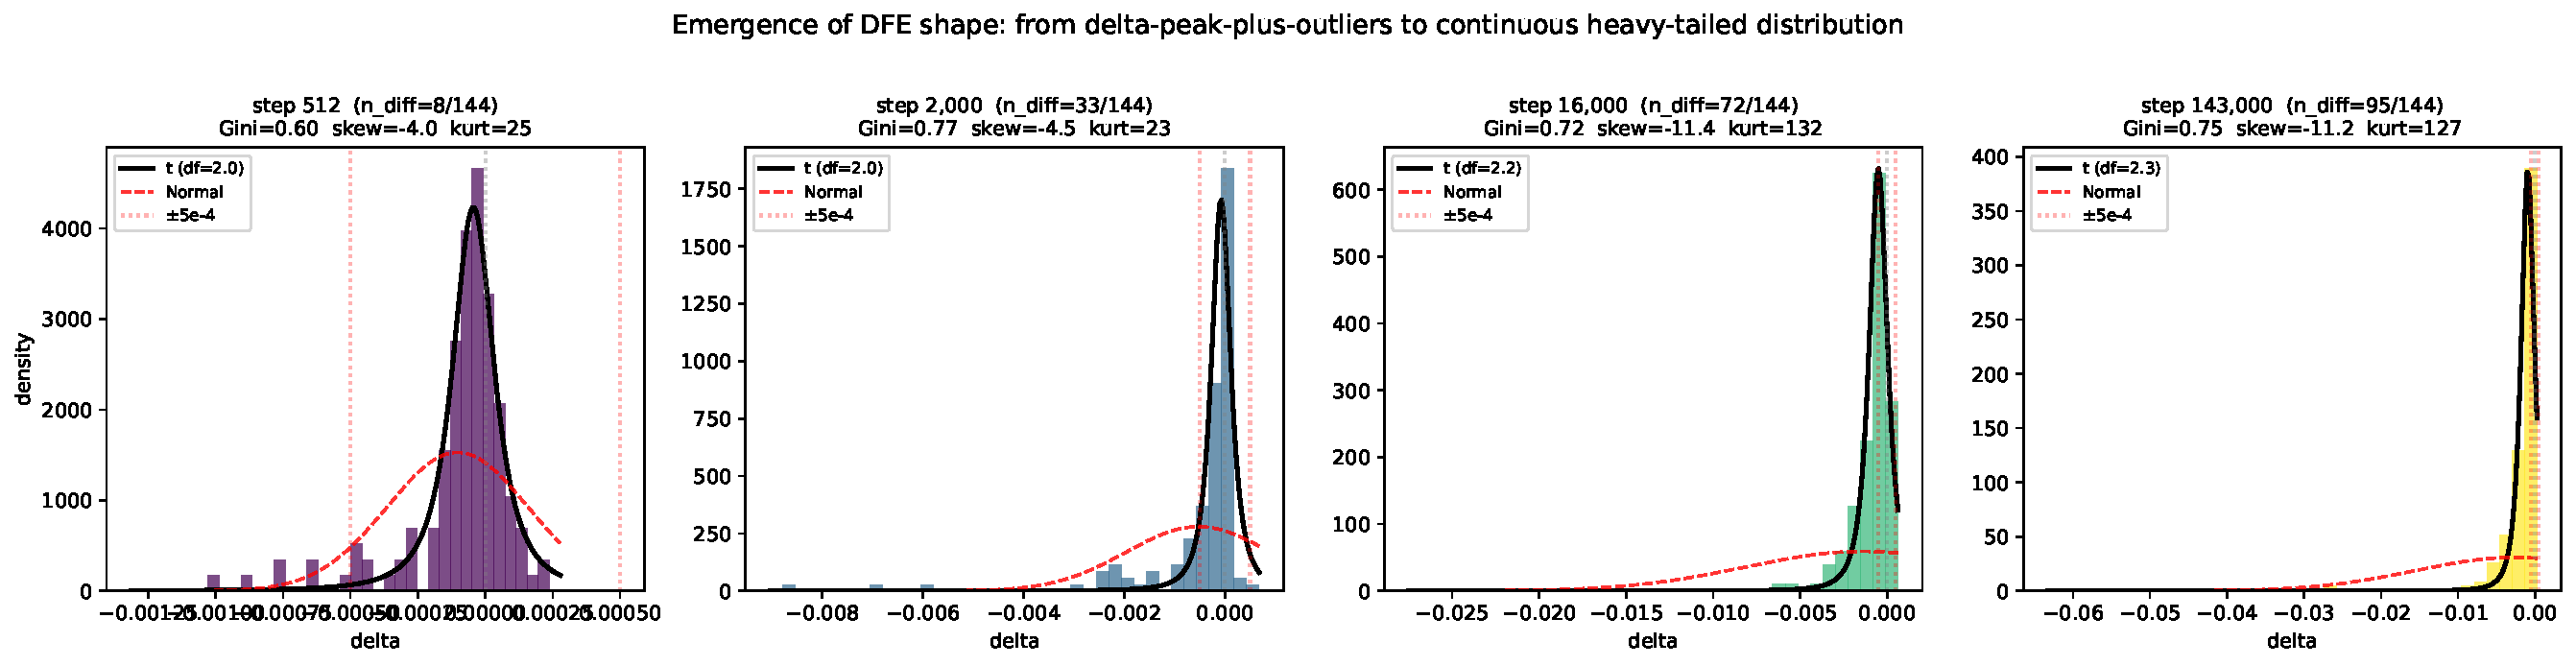
\includegraphics[width=0.95\textwidth]{figures/fig3_dfe_emergence.pdf}
    \caption{Distribution of fitness effects for 144 head ablations at four representative checkpoints. Histograms (bars), fitted Student's $t$ (black), fitted Normal (red dashed). \textbf{At step 512}, the distribution is dominated by a narrow peak at zero with two outliers; the Student's $t$ AIC advantage ($\Delta\text{AIC} = +140$) reflects outlier capture, not distribution shape. \textbf{By step 2{,}000}, a continuous heavy-tailed distribution has emerged. \textbf{At step 16{,}000 and step 143{,}000}, the Student's $t$ form with strong negative skew matches the universal DFE shape reported across biological and engineered adaptive systems \citep{spiro2026universal}. The gamma shape $\beta$ of the deleterious tail evolves from $\beta = 1.77$ [95\% CI: 1.23, 2.84] at step 512 into the biological range (\emph{E. coli} $\beta \approx 0.5$, yeast $\beta \approx 0.7$) by step 1{,}000 and remains there. Titles report $n_\text{diff}$ (heads above threshold $5 \times 10^{-4}$), Gini, skewness, and kurtosis.}
    \label{fig:dfe_emergence}
\end{figure}

\begin{figure}[t]
    \centering
    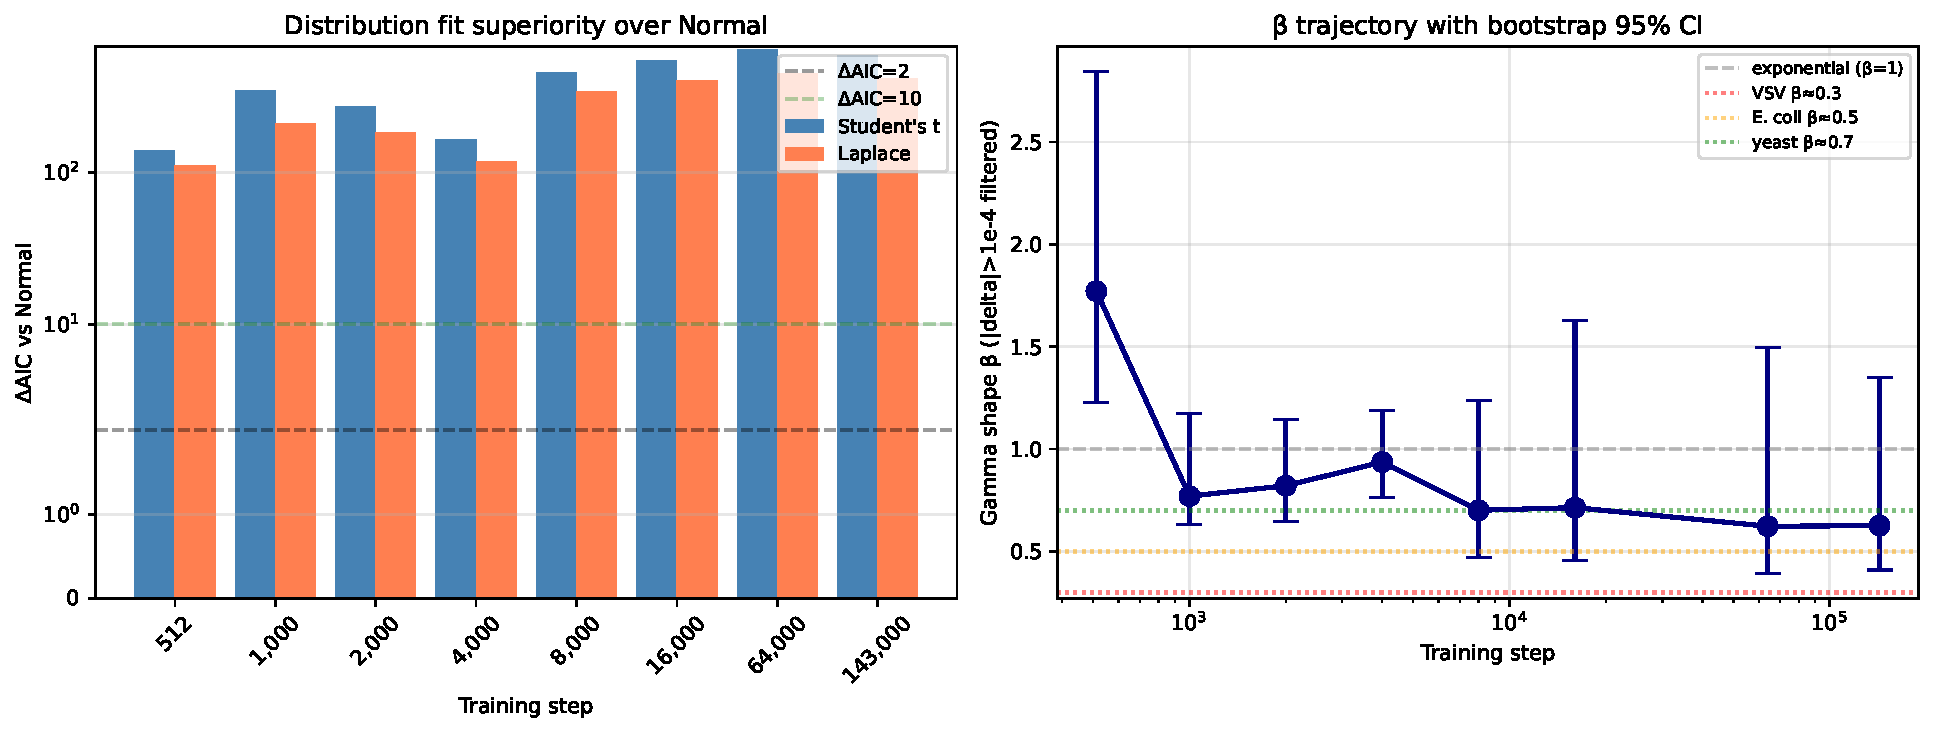
\includegraphics[width=0.95\textwidth]{figures/fig4_distribution_fits.pdf}
    \caption{\textbf{(a)} $\Delta\text{AIC}$ of Student's $t$ and Laplace distributions relative to Normal, at each checkpoint. Positive values indicate better fit than Normal. Student's $t$ decisively wins at every checkpoint ($\Delta\text{AIC} \gg 10$ throughout), confirming non-Gaussian shape. \textbf{(b)} Gamma shape parameter $\beta$ of the deleterious tail ($|\Delta| > 10^{-4}$ to exclude numerical noise), with 2{,}000-sample bootstrap 95\% CI. $\beta = 1.77$ at step 512 is in the light-tailed regime; the drop to $\beta \approx 0.8$ at step 1{,}000 is significant (non-overlapping CIs). Subsequent evolution to $\beta \approx 0.6$ at step 143{,}000 matches the biological range marked with dashed lines.}
    \label{fig:distribution_fits}
\end{figure}

Sections~\ref{subsec:emergence} and~\ref{subsec:dual} characterized the emergence of functional differentiation at the level of individual heads and at the level of the full 144-head distribution. We now turn to the shape of the DFE itself and ask whether the heavy-tailed Student's $t$ form reported by Paper~1 for mature adaptive systems is present throughout training, or whether the form itself emerges during training.

\textbf{The DFE shape transition is qualitative, not just quantitative.} Fig.~\ref{fig:dfe_emergence} shows the distribution of head-ablation effects at four representative checkpoints spanning the training trajectory: step~512, 2,000, 16,000, and 143,000. The visual transition is unambiguous. At step~512, the distribution is dominated by a narrow peak at zero with two outliers in the left tail --- there is no continuous tail; there is a delta-like mode with discrete excursions. By step~2,000, the peak has spread into a continuous distribution with visible mass across the negative range. At step~16,000 and step~143,000, the distribution has the characteristic shape reported in Paper~1 for mature adaptive systems: strongly left-skewed, heavy-tailed, well-fit by Student's $t$. This qualitative transition --- from delta-peak-with-outliers to continuous heavy-tailed distribution --- is the primary visual evidence that the universal DFE form is emergent rather than preformed.

\textbf{Student's $t$ fit is statistically preferred throughout, but its meaning changes.} Quantitative fits corroborate the visual reading with a subtlety. The AIC advantage of Student's $t$ over Normal is large at every checkpoint: $\Delta\text{AIC}(t \text{ vs } \mathcal{N}) = +140$ at step~512, $+347$ at step~1,000, $+275$ at step~2,000, $+589$ at step~143,000 (Fig.~\ref{fig:distribution_fits}a). Naively, this suggests the Student's $t$ form holds throughout. But the step-512 advantage is driven by outlier capture, not by a continuous heavy tail: Student's $t$ with $df \to 2$ fits any distribution with a narrow core plus two extreme observations better than Normal, even when the bulk is essentially a delta. The Student's $t$ fit is statistically preferred at all checkpoints, but what it fits \emph{means} different things at different checkpoints --- at step~512, it fits an outlier regime over an otherwise-concentrated bulk; at step~16,000 and beyond, it fits a continuous heavy-tailed distribution that spans the full range of head effects. The continuous-tail interpretation at step~143,000 is supported by the sensitivity analysis in Sec.~\ref{subsec:hierarchy}: Student's $t$ $df$ remains essentially unchanged ($2.34 \to 2.33$) after removing the five most extreme head ablations, confirming that the heavy-tailed fit captures population-level structure rather than outlier events at mature checkpoints. This contrasts with step~512, where the fit is necessarily outlier-driven because the bulk of the distribution is concentrated below the numerical floor. Fig.~\ref{fig:dfe_emergence} makes this distinction visible at the distribution level; the AIC number alone does not.

\textbf{Median gamma shape $\beta$ moves into the biological range.} The gamma shape parameter $\beta$, fit to the deleterious tail ($|\Delta| > 10^{-4}$ to filter the numerical floor), provides a more sensitive quantitative reading. The median bootstrap $\beta$ value declined from $1.78$ at step~512 to $0.62$ at step~143{,}000 (Fig.~\ref{fig:distribution_fits}b; 10{,}000 resamples). Bootstrap 95\% confidence intervals overlap between step~512 ($[1.22, 2.85]$) and step~143{,}000 ($[0.41, 1.35]$), so we do not claim statistical significance for the trajectory on this sample size. What we can claim, as an observation: \textbf{the median $\beta$ at step~512 lies above 1, in the near-exponential regime, while the median $\beta$ at step~143{,}000 lies below 1 in the heavy-tailed regime} --- specifically, within the biological range reported in Paper~1 for \emph{E. coli} ($\beta \approx 0.5$) and yeast ($\beta \approx 0.7$). The head-level DFE of the trained model shares a quantitative tail parameter with biological systems; the head-level DFE of the early-training model does not.

\textbf{The universal form is a property of trained systems.} Combining the preceding observations, we formulate the core finding of this section: the universal heavy-tailed DFE form documented by Paper~1 is not present at early training and emerges within the first few thousand steps of training. For Pythia 410M, the qualitative transition from pre-emergence DFE (delta-peak-with-outliers) to post-emergence DFE (continuous heavy-tailed) is substantially complete by step~1,000--2,000 --- within the first few thousand training steps. Subsequent training continues to refine the shape within the post-emergence regime ($\beta$ fluctuates in the range 0.6--0.9 between step~1,000 and step~143,000, skewness deepens as individual heads like L8H9 emerge; see Sec.~\ref{subsec:l8h9}), but the qualitative distributional structure is in place very early. This refines Paper~1's substrate-independence claim along the temporal axis: \textbf{the universal form applies to mature adaptive systems; the emergence of the form is a separate phenomenon with its own structure}, described by Secs.~\ref{subsec:emergence}--\ref{subsec:dual} and~\ref{subsec:hierarchy}.

\subsection{Iterable scale hierarchy of perturbations}
\label{subsec:hierarchy}

\begin{figure}[t]
    \centering
    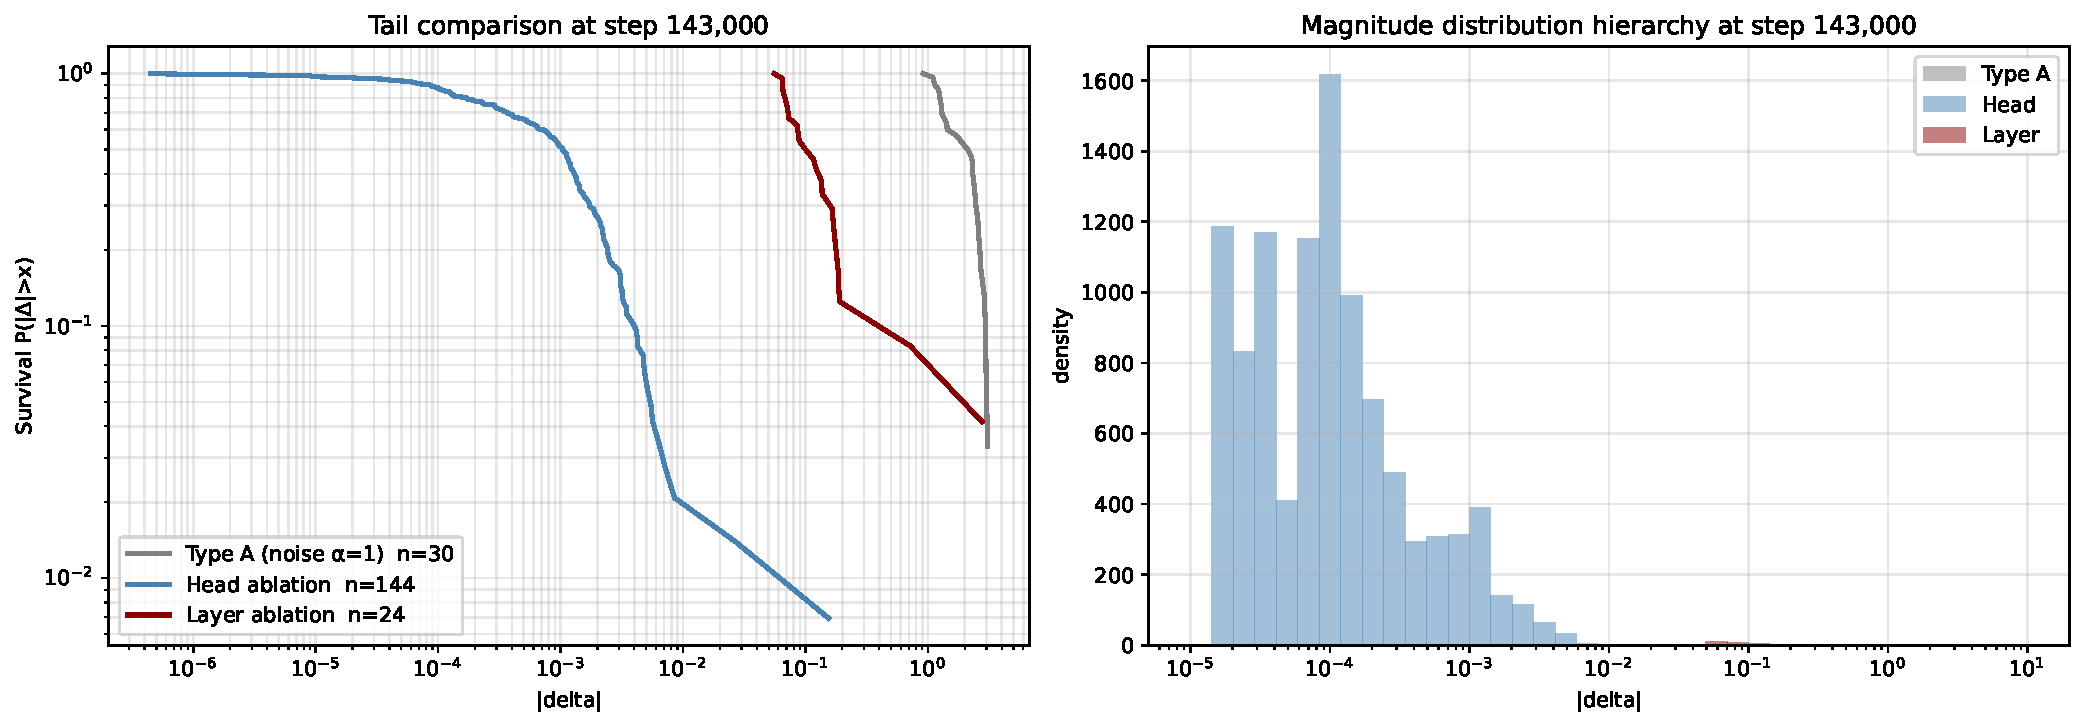
\includegraphics[width=0.95\textwidth]{figures/fig6_hierarchy.pdf}
    \caption{Ablation effect distributions at step 143{,}000 for three perturbation granularities: distributed parametric noise ($\alpha = 1 \cdot \sigma$ applied to all parameters of one block, $n = 30$), single attention head ablation ($n = 144$), single transformer layer ablation ($n = 24$). \textbf{(a)} Survival function $P(|\Delta| > x)$ on log-log axes. \textbf{(b)} Magnitude density on log $|\Delta|$ axis. Three qualitatively distinct regimes are observed, not points on a smooth heaviness gradient (see Table~\ref{tab:three_regimes}). Head-level ablation is the primary finding: a robustly heavy-tailed Student's $t$ distribution matching biological DFE form ($\beta \approx 0.6$, within the \emph{E. coli}--yeast range from Paper~1). The heavy-tailedness is stable under outlier removal ($df$ remains $2.34$ after dropping the top-5 extreme observations), indicating a population-level property. Layer-level heavy-tailedness at $n = 24$ is by contrast fragile: removing Layer~0 and Layer~5 collapses the fit to Gaussian, revealing that the apparent heavy tail at this granularity is driven by two structural outliers on an otherwise Gaussian base. Distributed noise obeys the CLT into Gaussian regardless of landscape structure. See Fig.~S3 for the full sensitivity analysis establishing these regime classifications. \textbf{The universal heavy-tailed DFE form of Paper~1 applies at intermediate discrete granularity, bracketed on both sides: distributed perturbations Gaussianize via CLT, very-coarse discrete ablations become dominated by a few structural outliers.}}
    \label{fig:hierarchy}
\end{figure}

\begin{table}[t]
\centering
\caption{Three qualitatively distinct DFE regimes at step 143{,}000 (cf. Fig.~\ref{fig:hierarchy}).}
\label{tab:three_regimes}
\begin{tabular}{llll}
\toprule
Perturbation & Student's $t$ $df$ & $\Delta$AIC vs Normal & Regime \\
\midrule
Distributed noise & $\to \infty$ & $-2$ & Gaussian (CLT limit) \\
Head ablation & 2.34 & $+589$ & \textbf{Heavy-tailed (population-level)} \\
Layer ablation & 0.85 & $+82$ & Outlier-plus-Gaussian-base \\
\bottomrule
\end{tabular}
\end{table}

Paper~1 reported a universal heavy-tailed DFE form across biological and engineered adaptive systems. Our finding in Section~\ref{subsec:dfe_shape} --- that this form emerges during training rather than being present at initialization --- raises an immediate question about the \emph{scope} of the universality: under what conditions on the perturbation does the universal form apply? We show here that three qualitatively distinct DFE regimes coexist in a single trained model, separated by the granularity of the perturbation unit. Only one of these regimes --- intermediate discrete ablations at the attention-head level --- exhibits the universal heavy-tailed form reported in Paper~1.

At step 143,000 we compared three perturbation granularities (Fig.~\ref{fig:hierarchy}):

\begin{itemize}
    \item \textbf{Distributed noise (Type~A)}: Gaussian noise with scale $\alpha\sigma$ added to every parameter in one randomly chosen transformer block, $\alpha = 1.0$; 30 samples.
    \item \textbf{Head ablation}: a single attention head zeroed via output-projection masking; 144 samples (our primary protocol).
    \item \textbf{Layer ablation}: all parameters of one transformer block zeroed; 24 samples (exhaustive).
\end{itemize}

Fit parameters and regime classifications:

\begin{center}
\begin{tabular}{llllllll}
\toprule
Perturbation & $n$ & std$(\Delta)$ & skew & excess kurt & $\Delta\text{AIC}(t \text{ vs } \mathcal{N})$ & Student's $t$ $df$ & Regime \\
\midrule
Distributed (Type~A) & 30 & 0.68 & $-0.10$ & $-1.5$ & $-2$ & $\to\infty$ & Gaussian (CLT limit) \\
Head (discrete, mid) & 144 & 0.013 & $-11.2$ & $+127$ & $+589$ & $2.34$ & \textbf{Heavy-tailed (robust)} \\
Layer (discrete, large) & 24 & 0.54 & $-4.2$ & $+16.7$ & $+82$ & $0.85$ & Outlier-plus-Gaussian base \\
\bottomrule
\end{tabular}
\end{center}

\textbf{Primary finding: head-level ablation DFE is robustly heavy-tailed and matches biological DFE form.} Head ablation at $n = 144$ produces a Student's $t$ distribution with $df = 2.34$ and $\Delta\text{AIC}$ = +589 against Normal. The gamma shape parameter of the deleterious tail, $\beta \approx 0.63$ (Sec.~\ref{subsec:dfe_shape}), falls within the biological range reported in Paper~1 for \emph{E. coli} ($\beta \approx 0.5$) and yeast ($\beta \approx 0.7$). This is the granularity at which substrate-independence holds most cleanly in our data: the heavy-tailed universal form is a \emph{population-level} property across many contributing heads, not the artifact of a few outliers.

\textbf{The three regimes are qualitatively distinct, not points on a smooth gradient.} A sensitivity analysis reveals a key structural difference between the two non-Gaussian regimes. For head ablations, the Student's $t$ $df$ is remarkably stable under outlier removal: $df = 2.34$ for $n = 144$, and $df = 2.33$ after removing the five most extreme $|\Delta|$ observations. The AIC advantage over Normal decreases with sample size (from $+589$ to $+8$ after removing the top-five) but the shape parameter does not drift. Many heads contribute to the tail; the distribution's heavy-tailedness is a population-level property. For layer ablations, by contrast, the heavy-tailedness is driven by two specific components: removing Layer~0 shifts $df$ from 0.85 to 1.74; removing both Layer~0 and Layer~5 collapses the fit to Gaussian ($df \to \infty$, $\Delta\text{AIC}(t \text{ vs } \mathcal{N}) = -2$). At step 143,000, Layer~0 ablation is dramatically more costly than any other layer ablation ($|\Delta|_{L_0} \approx 30\times$ the median of $L_1$--$L_{23}$), and Layer~5 is second-most costly ($\approx 8\times$ the median). The remaining 22 layers exhibit an approximately Gaussian distribution of ablation effects. Layer-level DFE at $n = 24$ is thus best described as an \emph{outlier-plus-base} regime --- two structural outliers on a Gaussian base of less-critical components --- rather than as a continuous heavy-tailed distribution. This distinction is itself a content finding: \textbf{robust heavy tails at intermediate granularity, outlier-dominated regime at very large granularity}. We speculate that this difference may generalize. As perturbation units approach the scale of entire functional subsystems (e.g. ablating all attention stacks, all MLP stacks, or specific multi-layer circuits), we expect distributions increasingly dominated by a small number of structurally critical units rather than smooth heavy tails. This is empirically testable and open-ended (Fig.~S3 reports the full sensitivity analysis).

The mechanism underlying the three regimes is straightforward. For distributed noise, each of roughly $3\!\times\!10^7$ parameters in a transformer block contributes a small, approximately independent effect on loss; by the central limit theorem, their sum tends to Gaussian regardless of the landscape geometry underlying any single parameter. For discrete-component ablations no such averaging applies. Each ablation is a single isolated event, and the shape of the resulting distribution reflects the intrinsic functional asymmetry of the components. At the head level, $n = 144$ samples span a rich functional diversity (Sec.~\ref{subsec:emergence}: a continuum from born-critical through emergent to never-critical heads), producing a continuous heavy tail. At the layer level, the 24 units are too few to populate the tail continuously, and the distribution is dominated by the handful of layers whose functional role is disproportionate.

This refines Paper~1's substrate-independence claim: \textbf{the universal heavy-tailed form is a property of the distribution of discrete component removals at an intermediate granularity where the number of functionally distinct units is large, not of arbitrary perturbations to parameter space}. Any distributed perturbation, in the limit of many contributing parameters, will appear Gaussian regardless of the landscape structure beneath it. Any ablation at a granularity too coarse relative to the system's functional hierarchy will show outlier-dominated structure, not a smooth heavy tail. The regime in which universality holds is bracketed on both sides. This distinction was implicit in Paper~1 --- all reported biological and engineered DFEs used discrete-unit perturbations at granularities natural to the system --- but was not formalized. We call the structure made explicit in Fig.~\ref{fig:hierarchy} an \emph{iterable scale hierarchy}: \emph{iterable} because the three points we measure are not exhaustive, and finer subdivisions (single-neuron ablation, cross-layer circuits, $N$-head joint ablation) would extend the hierarchy in either direction, each providing an empirical test of the regime boundaries sketched here.

\textbf{Second empirical witness for emergent differentiation.} A feature of the Type~A data that is not apparent from the step-143,000 snapshot above: distributed noise does not always produce a Gaussian DFE. At step~512, Type~A ablations are heavy-tailed ($\Delta\text{AIC}(t \text{ vs } \mathcal{N}) = +55$), decisively preferring Student's $t$. The transition to Gaussian occurs over the first $\sim\!2,\!000$ steps and is complete by step~4,000.

The mechanism mirrors head-level emergence (Sec.~\ref{subsec:emergence}). At step~512, Layer~0 ablation is dramatically more costly than any other layer ablation ($|\Delta|_{L_0} \approx 0.28$ versus typical $|\Delta| \sim 10^{-3}$ for other blocks), creating the heavy tail that Type~A noise inherits when it perturbs this layer disproportionately. As training progresses, all 24 blocks become individually important (Fig.~\ref{fig:layer_heatmap}), and the effective number of blocks that contribute non-negligibly to loss grows. The CLT then applies to distributed noise, and Type~A DFE Gaussianizes.

This is an \textbf{independent witness of the broadening component of dual differentiation} (Sec.~\ref{subsec:dual}): the number of functionally active blocks increases during training, measured not via head ablation but via the \emph{transition of the Type~A distribution from heavy-tailed to Gaussian}. Head-level and block-level trajectories move in opposite distributional directions --- head DFE becomes heavier-tailed, distributed-noise DFE becomes lighter --- yet both witness the same underlying process.

\begin{figure}[t]
    \centering
    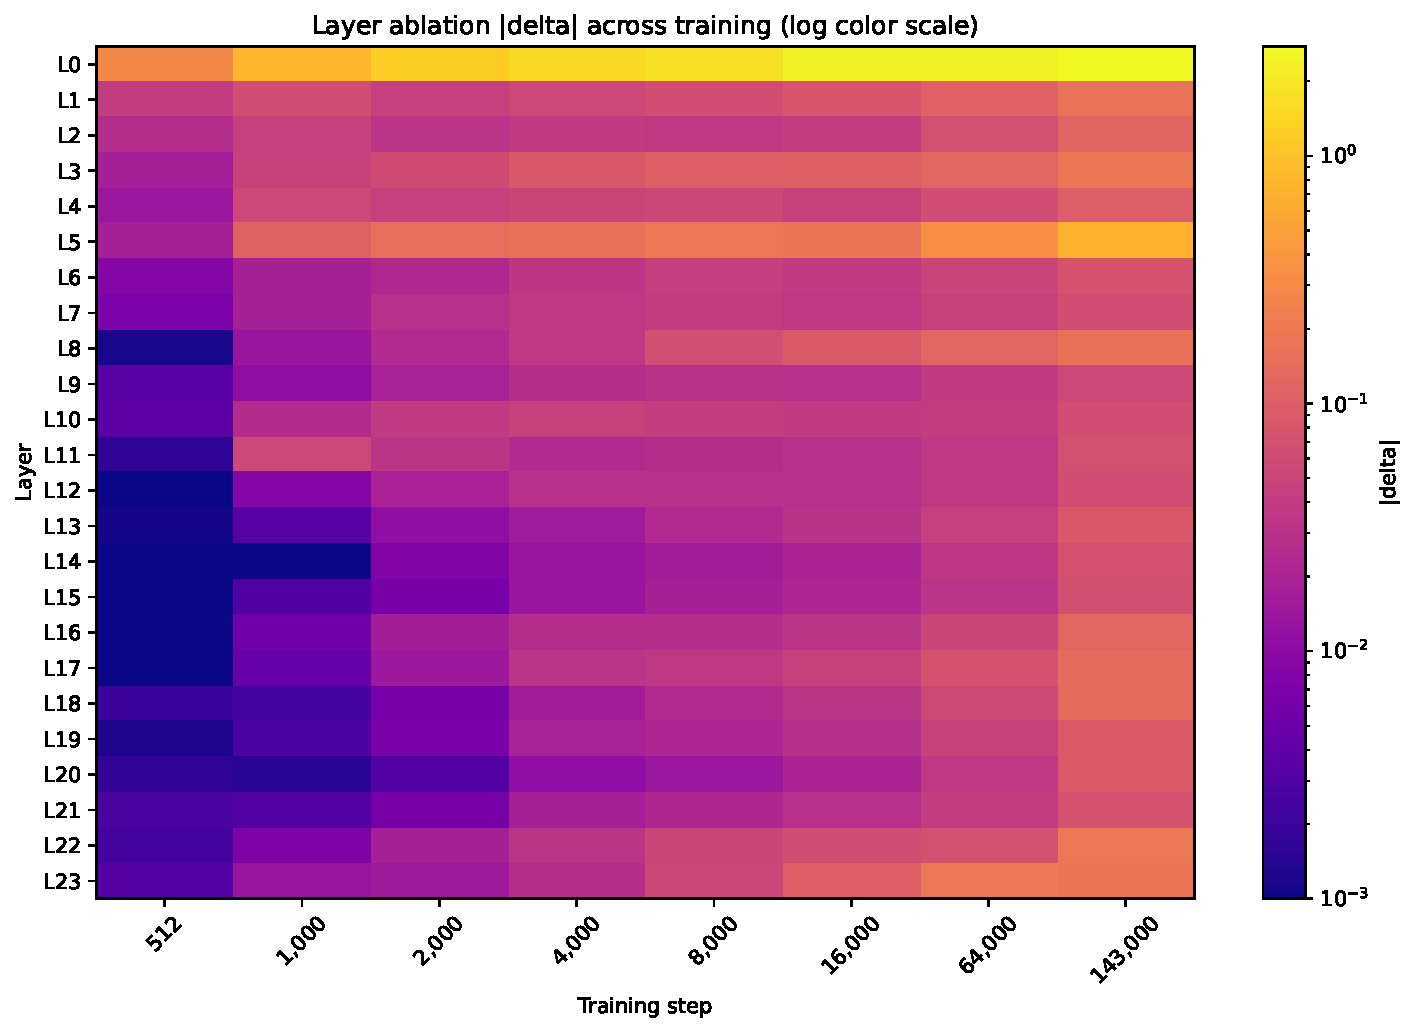
\includegraphics[width=0.9\textwidth]{figures/fig5_layer_heatmap.pdf}
    \caption{Heatmap of $|\Delta|$ for all 24 layer ablations across 8 checkpoints (log color scale). \textbf{Layer 0 is the dominant critical component at every checkpoint} --- removing it grows in impact from $|\Delta| = 0.28$ (step 512) to $|\Delta| = 2.76$ (step 143{,}000). Layer 5 is second in importance, growing from $0.018$ to $0.71$; the L0/L5 ratio shrinks from $15.9$ to $3.9$, indicating L5 catches up to L0 in relative criticality. Middle layers (L9--L15) remain the least critical throughout. The monotonic darkening at every layer confirms that total dependency on every discrete unit increases during training --- a layer-level analog of the head-level differentiation.}
    \label{fig:layer_heatmap}
\end{figure}

\subsection{Case study: L8H9 crystallization}
\label{subsec:l8h9}

\begin{figure}[t]
    \centering
    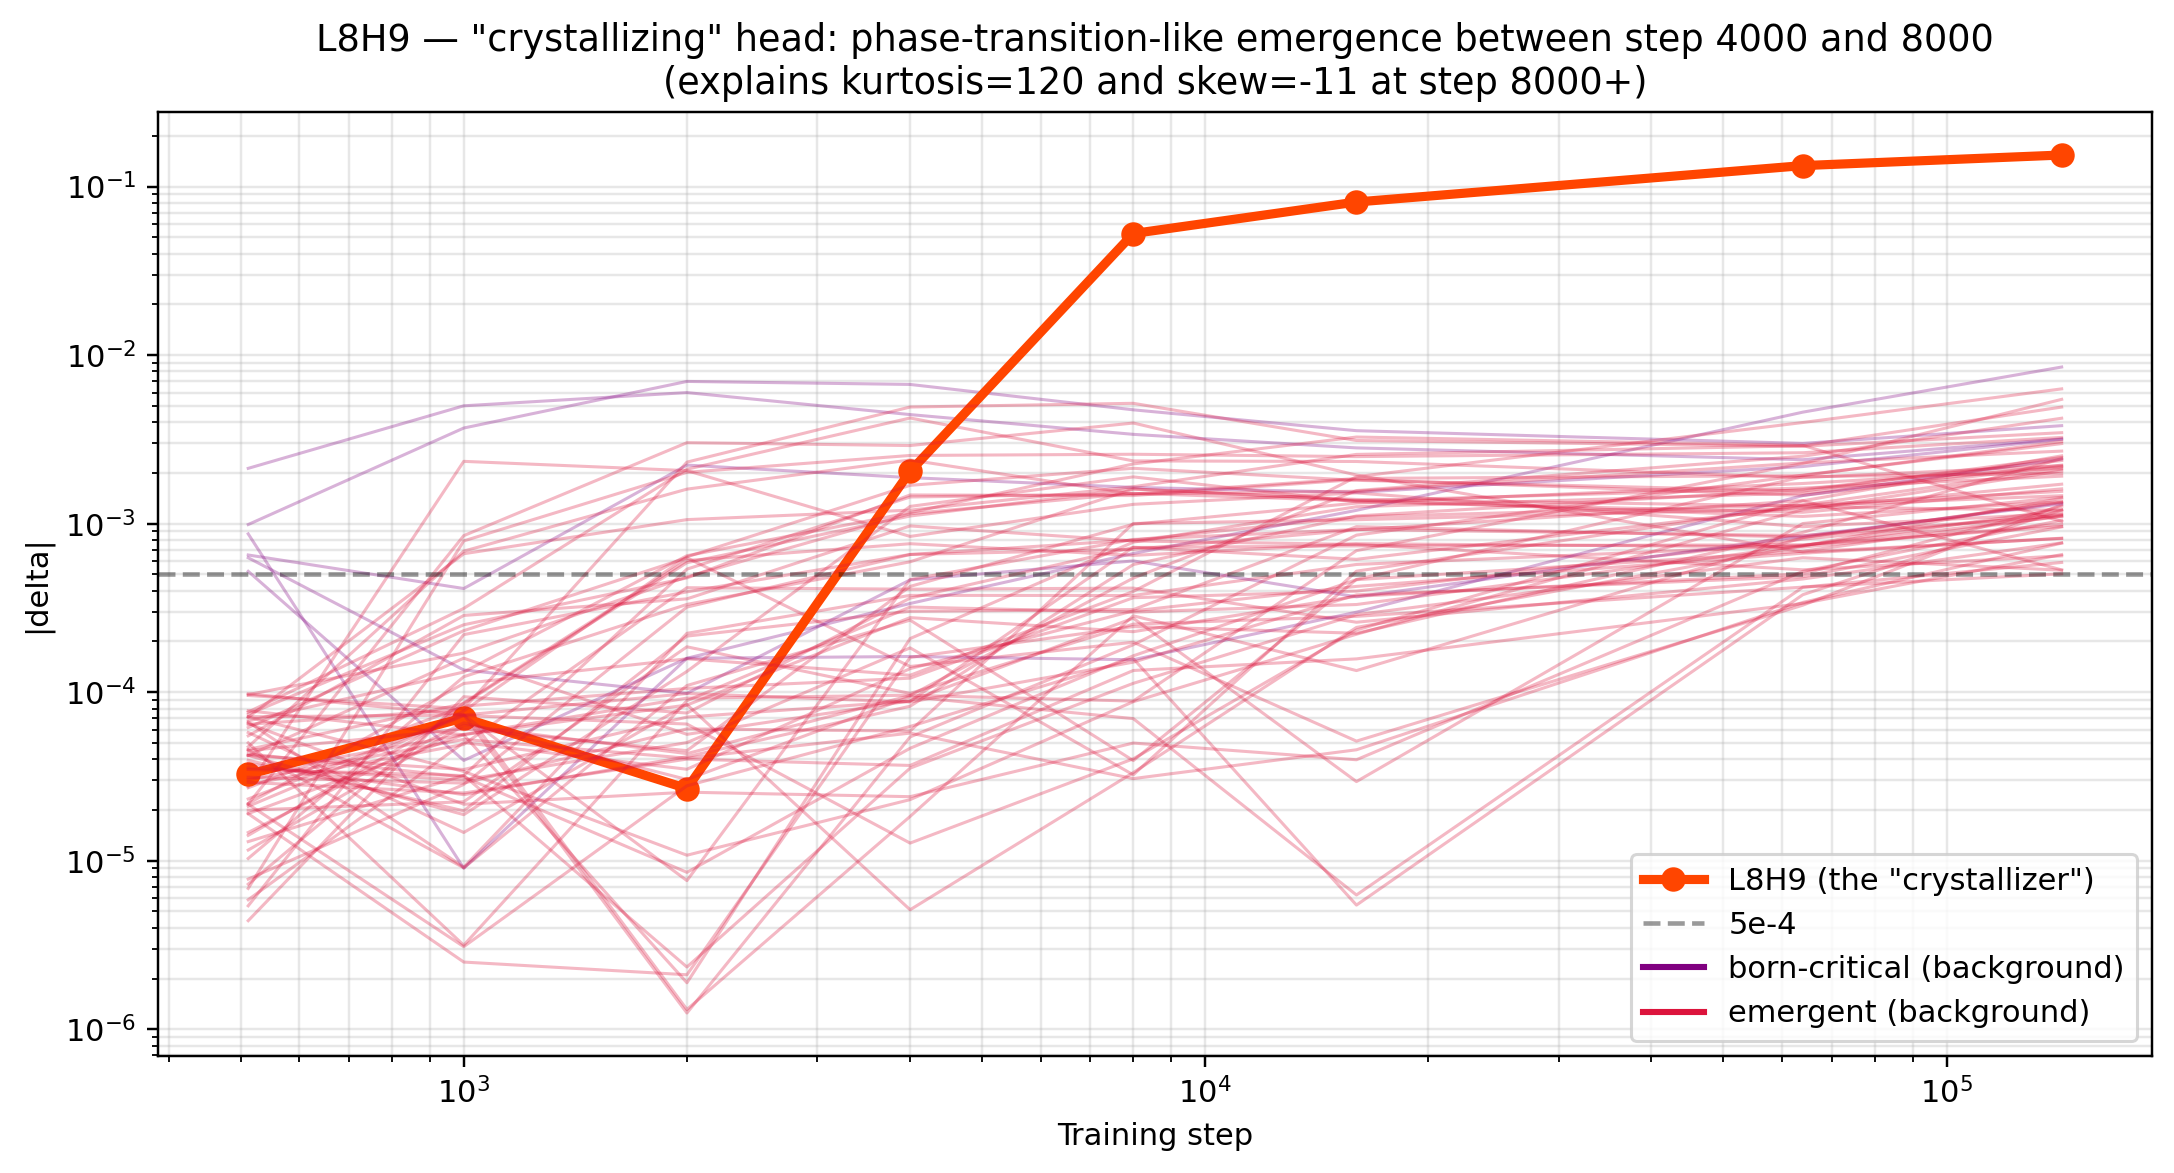
\includegraphics[width=0.9\textwidth]{figures/fig7_L8H9_crystallization.png}
    \caption{Absolute effect of ablating Layer 8 Head 9 across training (orange, heavy), overlaid on trajectories of other born-critical and emergent heads (gray background). Between step 4{,}000 and step 8{,}000, L8H9's ablation effect jumps by more than $20 \times$ (from $2 \times 10^{-3}$ to $5.3 \times 10^{-2}$) and continues growing to $1.54 \times 10^{-1}$ by step 143{,}000 --- approximately $5.7 \times$ the second-most-critical head. This single emergence dominates the kurtosis $\approx 127$ signal observed at step $8{,}000+$ (Fig.~\ref{fig:distribution_fits}a). The step-$4{,}000$-to-$8{,}000$ phase-transition-like emergence is a concrete target for mechanistic-interpretability follow-up: identifying the specific computation that crystallizes in L8H9 during this interval would link our component-level quantitative measurement to a circuit-level qualitative understanding.}
    \label{fig:l8h9}
\end{figure}

We close the results with a single-head case study for two reasons: to ground the population-level claims of Sections~\ref{subsec:emergence}--\ref{subsec:dfe_shape} in a concrete identifiable component, and to identify a specific target for mechanistic follow-up.

Section~\ref{subsec:emergence} identified 56 heads in the emergent class --- heads that transitioned from below the numerical noise floor at step~512 to functional criticality by step~143,000. One head in this class, Layer 8 Head 9 (L8H9), stands out as the most extreme instance of emergence in our sample: at step~143,000, its ablation effect is approximately $5.7\times$ the second-most-critical head and $\sim\!25\times$ the median of the ten most critical heads. \textbf{L8H9 exemplifies, rather than constitutes, the emergent class.} Fifty-five other heads in our sample underwent qualitatively similar transitions, most with smaller final magnitudes; we focus on L8H9 for the clarity of its signature, not its uniqueness.

\textbf{Phase-transition-like trajectory.} L8H9's ablation effect across the 8 tracked checkpoints (Fig.~\ref{fig:l8h9}):

\begin{center}
\begin{tabular}{lcccccccc}
\toprule
step & 512 & 1{,}000 & 2{,}000 & 4{,}000 & 8{,}000 & 16{,}000 & 64{,}000 & 143{,}000 \\
\midrule
$|\Delta|$ & $3{\times}10^{-5}$ & $1{\times}10^{-4}$ & $3{\times}10^{-6}$ & $2{\times}10^{-3}$ & $\mathbf{5.3{\times}10^{-2}}$ & $8.1{\times}10^{-2}$ & $1.3{\times}10^{-1}$ & $1.5{\times}10^{-1}$ \\
\bottomrule
\end{tabular}
\end{center}

From step~512 through step~2,000, L8H9 ablation produces effects indistinguishable from the numerical noise floor ($|\Delta| < 10^{-4}$). Between step~2,000 and step~4,000, an effect of approximately $2 \times 10^{-3}$ emerges. Between step~4,000 and step~8,000, $|\Delta|$ jumps by more than $20\times$ in a single checkpoint interval, from $2 \times 10^{-3}$ to $5.3 \times 10^{-2}$. This factor-of-$20$ increase within a factor-of-two increase in training steps is among the sharpest interval-over-interval growth rates observed in our 144-head sample. Beyond step~8,000, $|\Delta|$ continues to grow by a further $\sim\!3\times$ over the remaining $\sim\!95\%$ of training (by step count). We describe this pattern as \emph{phase-transition-like} in the descriptive sense: a rapid reorganization concentrated in a short interval of training, flanked by slower evolution on either side. We use the term as metaphor, not as a technical invocation of critical-point scaling.

\textbf{Distribution-level signature of a single-head event.} L8H9's emergence is visible in population-level DFE statistics at the same step as its crystallization. At step~4,000 (before the jump), the head-ablation distribution has skewness $-3.4$ and excess kurtosis $+13.7$. At step~8,000 (after the jump), skewness deepens to $-10.7$ and excess kurtosis to $+121$ --- a roughly factor-of-$9$ change in kurtosis within a factor-of-two change in training steps. These extreme values persist through step~143,000 (skewness $-11.2$, kurtosis $+127$). 

Importantly, the \emph{shape} parameter of the population-level fit --- Student's $t$ $df$ --- is unchanged by L8H9's presence: removing L8H9 from the step-143,000 distribution leaves $df = 2.34$ essentially unchanged (Sec.~\ref{subsec:hierarchy}). L8H9 drives the extreme-tail \emph{moments} (skewness and kurtosis, which are dominated by the single largest observation) but not the overall \emph{shape}, which is a population-level property across many contributing heads. L8H9 is the most visible tip of a broader emergent class that collectively determines the distributional shape; it is not a single-point driver of the universal form. The sensitivity result thus resolves what would otherwise be an interpretive ambiguity: extreme skewness and kurtosis at step~8,000+ could be caused by one extreme outlier on an otherwise-light distribution, or by a genuine heavy tail containing one extreme instance. The head-level $df$ stability (Sec.~\ref{subsec:hierarchy}) establishes the second reading.

\textbf{Open questions for mechanistic interpretability.} We identify L8H9 as a target for mechanistic analysis but do not claim to know its computational function. The specific computation L8H9 implements in the mature model, and the specific weight-space changes during the step-$4{,}000$-to-$8{,}000$ interval that produce that computation, remain open. A natural follow-up experiment is activation patching between step~4,000 and step~8,000 --- comparing mature-model behavior against pre-crystallization behavior --- to identify which inputs and which downstream targets change most under the ablation of L8H9, and which weight-level changes within this interval are responsible. This would connect our quantitative component-level measurement to circuit-level qualitative understanding in the style of recent mechanistic interpretability work \citep{olsson2022induction, wang2023interpretability, conmy2023automated}. We note that the single-model nature of our study does not establish whether the crystallization of L8H9 --- or of any specific head --- reproduces across Pythia sizes or other architectures; a scaling replication is a separate follow-up.

\textbf{Cross-dataset robustness.} To verify that L8H9's importance is not specific to wikitext-103, we measured its ablation effect at step 143{,}000 on three diverse evaluation sets: wikitext-103 ($|\Delta| = 0.154$), Colossal Common Crawl C4 English ($|\Delta| = 0.065$), and OpenWebText ($|\Delta| = 0.070$). L8H9 ablation increases loss substantially on every dataset tested, and remains the most impactful single-head ablation on all three. The magnitude varies by approximately $2\times$ across datasets, with wikitext-103 showing the largest relative effect; disentangling dataset-specific normalization effects (wikitext-103 has a lower baseline loss of $2.89$ than C4 at $3.06$) from content-specific encoding is a follow-up question beyond the scope of this single-checkpoint comparison. The consistency of L8H9 as the dominant single-head ablation across all three datasets is the point here. We attempted evaluation on Pile-validation and BookCorpus as well, but download links were not accessible from our Colab environment during this analysis; extending the comparison to these standard benchmarks is planned for future replication (Table~\ref{tab:tier1_l8h9_datasets}).

\textbf{L8H9 as the single-head view of Fig.~1.} Fig.~\ref{fig:head_trajectories} displays the functional differentiation of 144 heads at the population level. L8H9 is one of those 144 trajectories, specifically the steepest in the log-log view. The crystallization seen cleanly in L8H9's single-head trajectory (Fig.~\ref{fig:l8h9}) is the single-component version of the population-level phenomenon visible in Fig.~\ref{fig:head_trajectories}. Sec.~\ref{subsec:emergence} and Sec.~\ref{subsec:l8h9} describe the same process at two resolutions: Fig.~\ref{fig:head_trajectories} shows \emph{that} functional differentiation happens and at what scale; Fig.~\ref{fig:l8h9} shows \emph{what it looks like} for a specific emerging component. Functional differentiation is simultaneously a distributional pattern and a nameable event.

\section{Discussion}
\label{sec:discussion}

We summarize the four findings and then address their implications for the adjacent literatures, the diagnostic uses, the open questions, and the limitations.

\subsection{Relation to Paper~1: refinement, not contradiction}

Paper~1 reported substrate-independence of the DFE form across mature adaptive systems: biological mutations, architectural ablations in trained neural networks, and related engineered systems. Our work does not contradict this; it \emph{deepens} it by identifying the conditions under which the universality holds.

First, along the temporal axis: the universal heavy-tailed Student's $t$ form is a property of \emph{trained} systems, not of systems at initialization. In Pythia 410M, the qualitative transition from the pre-emergence regime (delta-peak-with-outliers) to the post-emergence regime (continuous heavy-tailed distribution) completes within the first $\sim\!1{,}000$--$2{,}000$ training steps (Sec.~\ref{subsec:dfe_shape}). Paper~1's biological and engineered examples were all mature systems, so this temporal condition was satisfied by construction but not recognized as a condition.

Second, along the granularity axis: the universal form applies to \emph{discrete modular} perturbations at an intermediate scale, not to arbitrary perturbations of the parameter space. Distributed perturbations obey the central limit theorem and Gaussianize regardless of the underlying landscape (Sec.~\ref{subsec:hierarchy}). Very-coarse discrete perturbations (at the layer level in our data) can produce distributions dominated by a small number of structural outliers rather than smooth heavy tails. The universal form occupies a regime of intermediate discreteness. Paper~1's biological examples used such intermediate-scale perturbations (single mutations, single ablations) implicitly; making this condition explicit is a non-trivial refinement.

Third, as a generative mechanism: Paper~1 gave no account of \emph{why} the universal form appears where it does. Our Sec.~\ref{subsec:emergence}--\ref{subsec:dual} propose that the form is generated by \emph{functional differentiation} of components during training. At every step, a growing fraction of heads cross the threshold above numerical noise and participate in the loss, while a shrinking effective number concentrates the bulk of importance in a few heads; the resulting population of importance values has the universal heavy-tailed shape. This is a mechanism at the population level; whether an analogous mechanism drives DFE universality in biology --- component-level differentiation during development, developmental canalization --- is a testable question, not a claim of this paper.

\subsection{Biological parallels}

Functional differentiation is a canonical biological concept. The trade-off between division of labor (broadening: more components with distinct functions) and specialization (concentration: few components carrying disproportionate roles) is studied in cell types \citep{wagner2014arrival}, microbial communities, developmental biology, and economic systems. Our dual differentiation conjecture provides the first \emph{quantitative simultaneous} measurement of both effects in an artificial system, using substrate-independent metrics (Gini coefficient, Hill number of order 1) that directly import biological diversity theory \citep{hill1973diversity, jost2006entropy}.

A specific testable prediction: \emph{in longitudinal biological development data, the same three-metric signature (count $\uparrow$, effective $N \downarrow$, Gini approximately invariant) should appear during cell fate differentiation in organogenesis}. Single-cell atlases of developing organs provide the data; we have not run this analysis here, and we frame it as a follow-up rather than as an established parallel.

\subsection{Gifts for adjacent communities}

Three findings open concrete follow-up directions for other research programs.

\textbf{For mechanistic interpretability.} The phase-transition-like emergence of L8H9 (Sec.~\ref{subsec:l8h9}, Fig.~\ref{fig:l8h9}) gives a specific target: which computation does L8H9 implement in the mature model, and what specific weight-space changes during the step-4{,}000-to-8{,}000 interval produce this computation? Activation patching between checkpoints in this interval, applied to L8H9 specifically, would reveal the crystallizing function. We provide the quantitative component-level identification; the circuit-level qualitative description is a follow-up for groups working in the tradition of \citet{olsson2022induction, wang2023interpretability, conmy2023automated}.

\textbf{For the lottery ticket / pruning community.} The 6 heads in the born-critical class are identifiable by index (Table~S1 lists top-10 critical heads at step 143,000; the intersection with critical heads at step 512 identifies the born-critical six). These heads were critical at step~512 and remained so through step~143,000. What structural feature of their initialization --- weight magnitude, attention-pattern statistics, position in the layer --- predicts their sustained criticality? Fig.~\ref{fig:layer_heatmap} already hints at a layer-position effect: Layers 0 and 5 dominate layer-level importance throughout training. The born-critical heads' distribution across layer positions is a natural starting point for a structural-predictor analysis. This is a direct test of lottery-ticket predictions at head granularity, not at parameter granularity \citep{frankle2019lottery}.

\textbf{For functional-redundancy research.} The 49 heads in the never-critical class remained below the $5 \times 10^{-4}$ threshold at every checkpoint. Are these heads truly null (carrying no information), or parallel-redundant (carrying information that adjacent heads duplicate, rendering single-head ablation ineffective)? This is a concrete question that $N$-head ablation protocols (ablating 2 or 3 never-critical heads simultaneously) can resolve. The answer has implications for the minimal functional complement of a trained transformer.

\subsection{Predictions for training diagnostics}

Our dual differentiation conjecture generates three testable predictions about training health:

\begin{itemize}
    \item \textbf{Healthy training} maintains approximately stable Gini ($\approx 0.7$ in Pythia 410M; specific values expected to differ by model and task) after the pre-emergence transition.
    \item \textbf{Collapsed representations} --- models where all function concentrates in one or a few components without growing a functional base --- should show Gini $\to 1$, the Lorenz curve approaching the corner. This predicts a training-health diagnostic complementary to loss-based metrics.
    \item \textbf{Undertrained or uniform networks} --- models that fail to differentiate their components --- should show Gini $\to 0$, the Lorenz curve approaching the diagonal.
\end{itemize}

These predictions are testable on known-pathological training runs (e.g., mode collapse events, runs interrupted mid-training, deliberately-degraded architectures). A successful test in any such case would upgrade the conjecture toward a diagnostic principle; failure would constrain dual differentiation to specific training regimes. We note that deliberate testing of these predictions would require access to pathological training runs, which are relatively rare in public model releases. A partial test is nonetheless possible using naturally-occurring variation in training quality --- for example, comparing Pythia checkpoints from interrupted versus completed training runs, or comparing the same architecture trained on different-quality data, if such data becomes available.

\subsection{Limitations}

We are explicit about what our single pilot does \emph{not} establish.

\begin{itemize}
    \item \textbf{Single model.} All results are obtained on Pythia 410M-deduped. We do not know whether the specific values (Gini $\approx 0.7$, $\beta \approx 0.63$, four-class distribution 4.2/38.9/22.9/34.0) generalize across sizes; whether the L8H9 crystallization has analogs at 1.4B or 12B; or whether the qualitative three-regime hierarchy (Gaussian / heavy-tailed / outlier-plus-base) transfers to other architectures.
    \item \textbf{Single task family.} Next-token prediction is one task domain. Vision models, RL agents, and multimodal models are not tested.
    \item \textbf{Single evaluation dataset.} All loss shifts are measured on wikitext-103. Cross-dataset replication would strengthen claims about the distribution shape.
    \item \textbf{Head-granularity sampling.} We ablated 144 of the model's 384 total attention heads. Finer sampling (full 384, or all parameters at sub-head resolution) might reveal sub-structure within our four classes.
    \item \textbf{$N$-head ablation not performed.} Single-head ablation cannot distinguish truly null heads from parallel-redundant heads. The 34\% never-critical class is under-resolved on this basis.
    \item \textbf{Upper bracket of universality regime empirically suggestive, not firmly established.} The "bracketed on both sides" framing in Sec.~\ref{subsec:hierarchy} treats layer ablation ($n = 24$) as the upper bracket. Strictly, this is suggestive: the collapse to outlier-plus-base regime could reflect the small sample size, not a genuine granularity effect. Measurements at intermediate granularities (multi-head circuits, single-MLP vs attention sub-block) would solidify this side of the bracket.
    \item \textbf{Temporal grid.} Our 8 checkpoints are log-spaced; finer temporal resolution around the emergence transition (particularly step 2,000--8,000) might reveal substructure.
    \item \textbf{Causal interpretation of emergence classes.} The born-critical / emergent / growing / never-critical classification is descriptive of trajectory patterns, not causal. Whether emergent heads become critical because they acquired specific functional content, or because redistribution of responsibilities during training forced them into critical roles, is not resolved by our measurements.
    \item \textbf{Potential wikitext--Pile leakage.} Our baseline loss is measured on wikitext-103, while Pythia was trained on the Pile, which includes Wikipedia content. Some overlap is possible in principle. As a sanity check we note that our wikitext-103 perplexity at step 143,000 ($\approx 18.0$) is substantially higher than published Pythia-410M Pile-validation perplexity ($\approx 10.2$, \citealp{biderman2023pythia}), indicating that wikitext is \emph{harder} than the training distribution for this model rather than easier; this is inconsistent with substantial train/test leakage. Our analysis depends on loss \emph{shifts} induced by ablations, not on absolute loss, and relative shifts are robust to moderate leakage. A systematic comparison with Pile-validation baselines is a straightforward follow-up check.
\end{itemize}

\subsection{Forward-looking}

The structure we call dual differentiation --- simultaneous broadening and concentration of function, with approximately invariant inequality --- is either a Pythia-specific phenomenon or a more general signature of how adaptive systems grow functional structure. Distinguishing these is the core of the natural follow-up program: scaling replication within the Pythia family (1.4B, 2.8B, 6.9B, 12B) tests size-invariance of the specific numerical signature; cross-architecture replication (OLMo, Llama, diffusion models) tests architecture-invariance; biological replication (single-cell trajectories during differentiation) tests substrate-invariance in the strongest form. The substrate-independent DFE framework of Paper~1 makes each of these tests quantitatively concrete: the same three metrics, the same statistical apparatus, the same conservation conjecture framing. This paper gives the apparatus a generative mechanism at the component level; the next papers test how far that mechanism extends.

Whether or not the conjecture holds beyond Pythia 410M, the empirical observation that functional differentiation is \emph{simultaneously a distributional pattern and a nameable event} --- that L8H9's phase transition and the population-level emergence visible in Fig.~\ref{fig:head_trajectories} describe the same phenomenon at different resolutions --- may itself prove a productive framing for future work. It shifts the question about universality from "does the form appear" to "what generates it, component by component".

\bibliographystyle{plainnat}
\bibliography{references}

\appendix

\section{Data and code availability}
\label{app:data}

All ablation data (1,584 rows) is available as CSV at \url{https://github.com/mool32/functional-differentiation-dfe}. The CSV fields are: \texttt{checkpoint}, \texttt{perturbation\_type}, \texttt{subtype}, \texttt{layer\_idx}, \texttt{head\_idx}, \texttt{seed}, \texttt{baseline\_loss}, \texttt{perturbed\_loss}, \texttt{delta}, \texttt{elapsed\_sec}. A self-contained Colab notebook reproducing the main sweep is included in the repository. Expected runtime on A100 40~GB: 82 minutes; compute cost approximately \$4.

\section{Supplementary figures}

\begin{figure}[h]
    \centering
    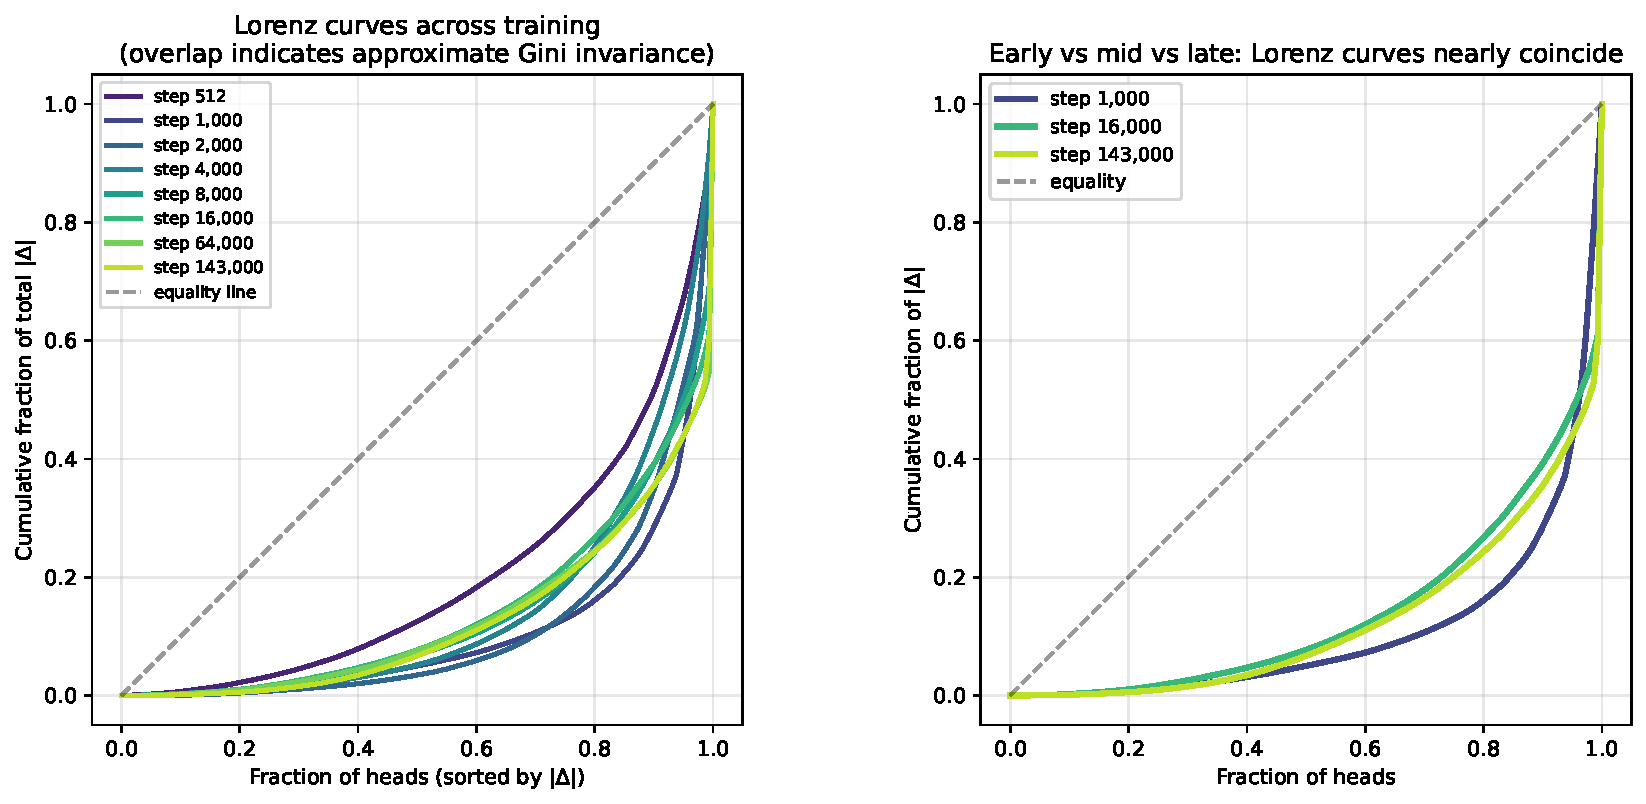
\includegraphics[width=0.95\textwidth]{figures/figS1_lorenz_curves.pdf}
    \caption{Lorenz curves of $|\Delta|$ distribution across 8 training checkpoints. Left: all checkpoints overlaid (viridis palette, earlier = darker). Right: three representative checkpoints (step 1{,}000, 16{,}000, 143{,}000). The near-coincidence of Lorenz curves from step 1{,}000 onward is the visual signature of approximate Gini invariance; step 512 (Gini $= 0.60$) is a distinct pre-emergence regime, consistent with the delta-peak-plus-outliers interpretation in Section~\ref{subsec:dfe_shape}.}
    \label{fig:lorenz}
\end{figure}

\begin{figure}[h]
    \centering
    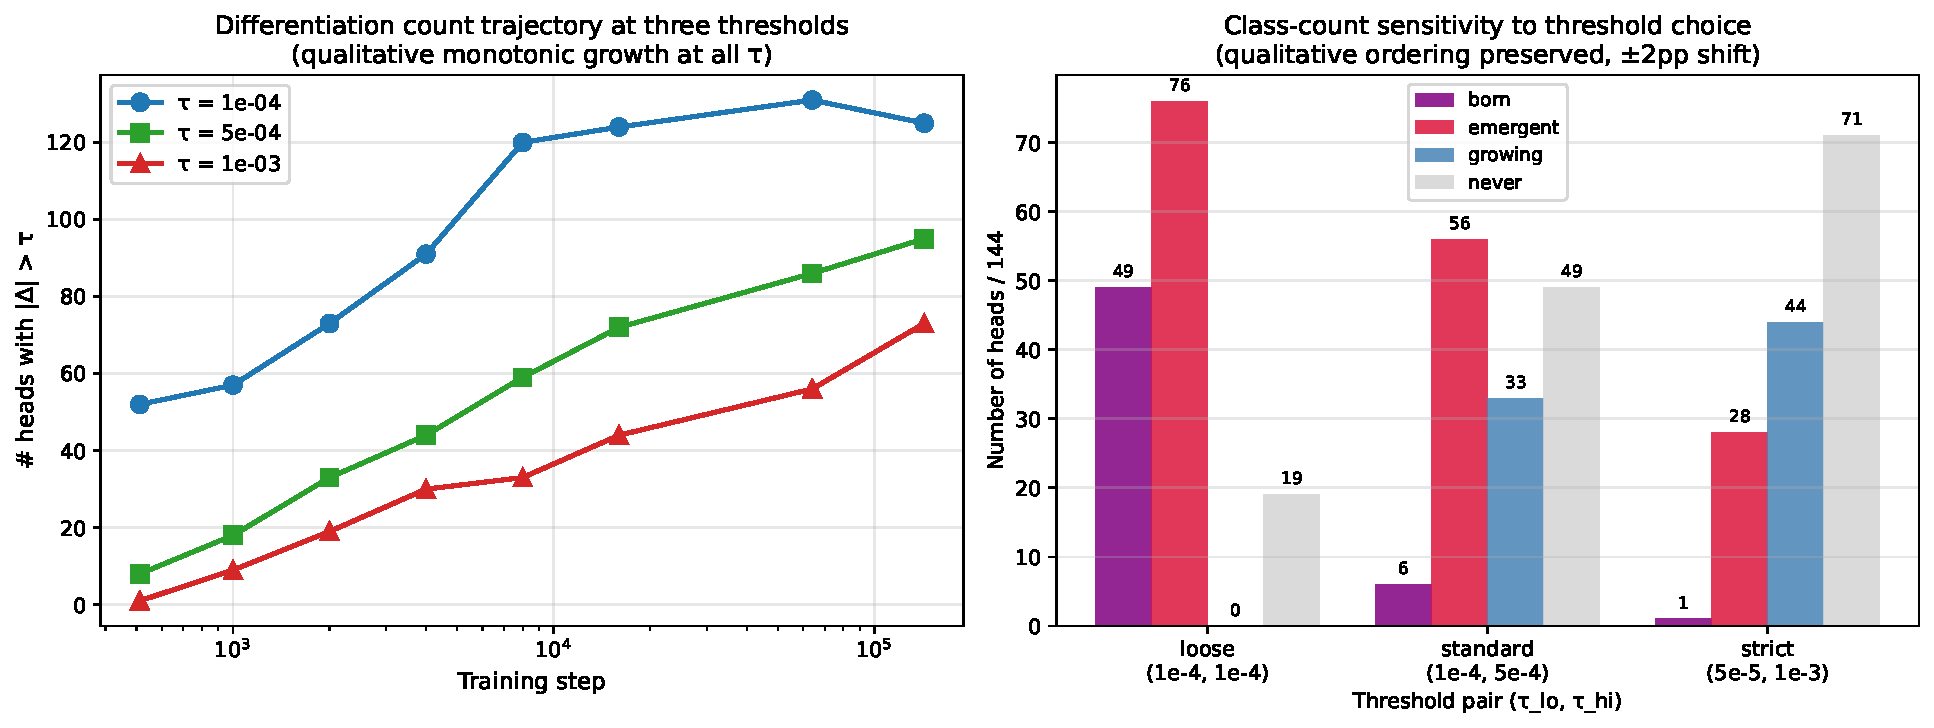
\includegraphics[width=0.95\textwidth]{figures/figS2_threshold_robustness.pdf}
    \caption{Robustness of differentiation count to threshold choice. (a) Per-checkpoint count of heads with $|\Delta| > \tau$ at three threshold values; the monotonic growth of the differentiation count is preserved at all tested thresholds. (b) Four-class classification counts under three threshold configurations; counts shift by at most $\pm 2$ percentage points, and the qualitative dominance of the emergent class over the born-critical class is preserved.}
    \label{fig:threshold_robust}
\end{figure}

\begin{figure}[h]
    \centering
    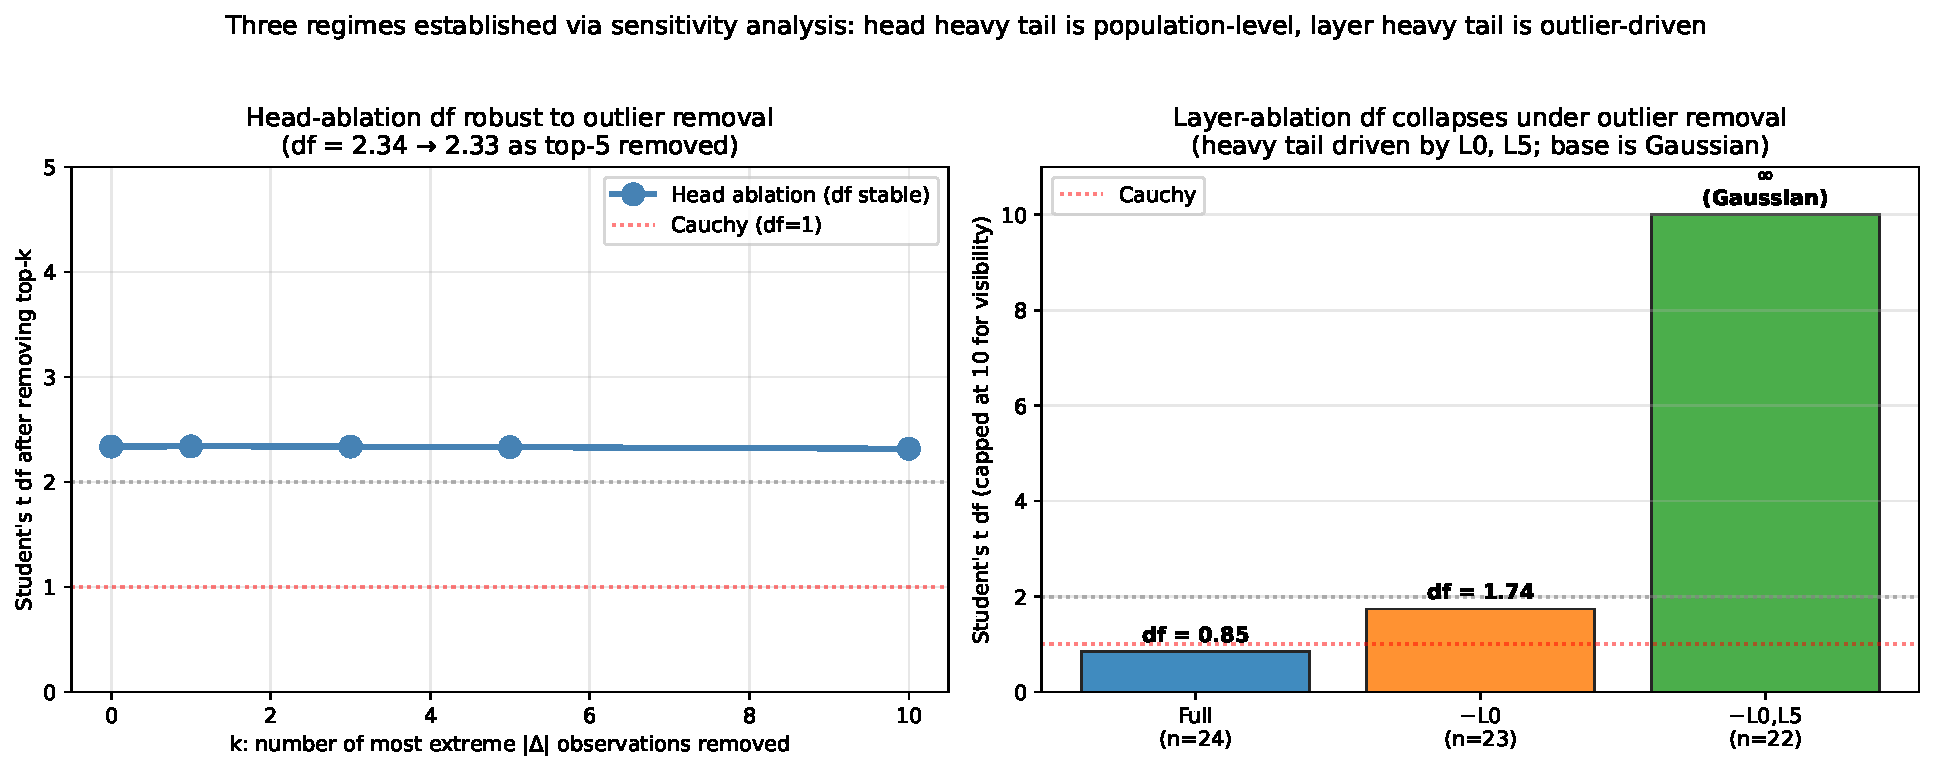
\includegraphics[width=0.95\textwidth]{figures/figS3_regime_sensitivity.pdf}
    \caption{Sensitivity analysis establishing the three DFE regimes of Fig.~\ref{fig:hierarchy}. (a) Head-ablation Student's $t$ $df$ is stable under outlier removal ($df = 2.34 \to 2.33$ after dropping top-5 most extreme observations), indicating a population-level heavy tail. (b) Layer-ablation $df$ drifts dramatically under outlier removal: dropping Layer~0 moves $df$ from $0.85$ to $1.74$; dropping Layer~0 and Layer~5 collapses the fit to Gaussian ($df \to \infty$). The layer-level heavy-tail is driven by two specific outliers on an otherwise Gaussian base.}
    \label{fig:regime_sensitivity}
\end{figure}

\begin{figure}[h]
    \centering
    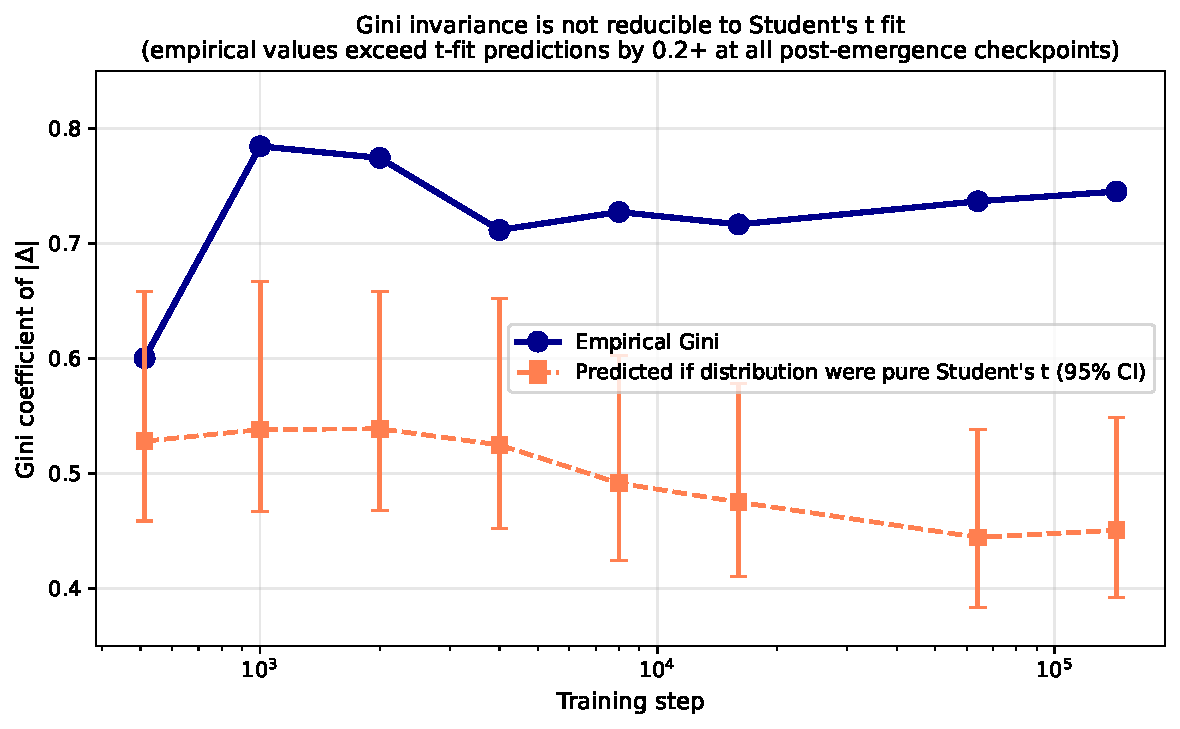
\includegraphics[width=0.95\textwidth]{figures/figS4_gini_triviality.pdf}
    \caption{Empirical Gini trajectory compared to the Gini predicted under a pure Student's $t$ null (95\% prediction interval from 2{,}000 samples per checkpoint of fitted-$t$-distributed values). Empirical Gini exceeds predicted by $\sim 0.2$ at all post-emergence checkpoints and falls outside the 95\% prediction interval at 7 of 8 checkpoints. Moreover, the predicted Gini declines across training while the empirical Gini is approximately stable, with cross-checkpoint correlation $r = -0.04$. The empirical Gini invariance is not a trivial consequence of the Student's $t$ fit.}
    \label{fig:gini_triviality}
\end{figure}

\section{Supplementary tables}

\begin{table}[h]
\centering
\caption{Top-10 most critical heads at step 143{,}000, ranked by $|\Delta|$.}
\label{tab:top10_heads}
\begin{tabular}{lcccccccccc}
\toprule
Rank & 1 & 2 & 3 & 4 & 5 & 6 & 7 & 8 & 9 & 10 \\
\midrule
Layer/Head & L8H9 & L4H6 & L0H9 & L1H6 & L12H0 & L16H15 & L7H0 & L13H6 & L8H6 & L4H9 \\
$|\Delta|$ & 0.154 & 0.0271 & 0.0085 & 0.0071 & 0.0063 & 0.0056 & 0.0055 & 0.0051 & 0.0049 & 0.0048 \\
Ratio to top-1 & 1.000 & 0.176 & 0.055 & 0.046 & 0.041 & 0.037 & 0.036 & 0.033 & 0.032 & 0.031 \\
\bottomrule
\end{tabular}
\end{table}

\begin{table}[h]
\centering
\caption{Drift monitoring on 500 consecutive ablate-restore cycles (Tier 1 T1.4). Single attention head (L5H7) ablated and restored 500 times; tensor SHA-256 hash compared to pre-ablation reference at every cycle; absolute-sum drift of the affected weight matrix recorded.}
\label{tab:tier1_drift}
\begin{tabular}{lr}
\toprule
Metric & Value \\
\midrule
Cycles & 500 \\
Initial $\sum |w|$ & 15{,}930.217 \\
Max drift observed & $0.0$ \\
Final drift & $0.0$ \\
Cycles with bitwise hash preserved & 500 / 500 \\
\bottomrule
\end{tabular}
\end{table}

\begin{table}[h]
\centering
\caption{Seed-replication of Type A perturbations across 8 checkpoints (Tier 1 T1.1). Comparison of std$(\Delta)$ obtained with original PRNG seed base 42{,}000 (Paper~2 main sweep) vs.\ alternate seed base 12{,}345 on an alternate 25-batch slice of wikitext-103 train. Ratio = std(alternate) / std(original); a ratio of 1.00 indicates perfect replication.}
\label{tab:tier1_seed}
\begin{tabular}{lrrr}
\toprule
Checkpoint & std (orig, seed 42000) & std (new, seed 12345) & Ratio \\
\midrule
512      & 0.03607 & 0.03513 & 0.974 \\
1{,}000  & 0.04924 & 0.04970 & 1.010 \\
2{,}000  & 0.03307 & 0.03308 & 1.000 \\
4{,}000  & 0.04048 & 0.03847 & 0.950 \\
8{,}000  & 0.06392 & 0.06127 & 0.959 \\
16{,}000 & 0.11820 & 0.11049 & 0.935 \\
64{,}000 & 0.31437 & 0.33096 & 1.053 \\
143{,}000 & 0.68400 & 0.69009 & 1.009 \\
\midrule
Mean ratio & & & 0.986 \\
Max deviation from 1.00 & & & 0.065 (6.5\%) \\
\bottomrule
\end{tabular}
\end{table}

\begin{table}[h]
\centering
\caption{Bootstrap convergence check for gamma shape $\beta$ (Tier 1 T1.3). Median and 95\% CI at 2{,}000 resamples (original analysis) vs.\ 10{,}000 resamples (used in paper). CI width ratio = width(10k) / width(2k).}
\label{tab:tier1_bootstrap}
\small
\begin{tabular}{lrrrrrrr}
\toprule
Checkpoint & $\beta_{2k}$ median & $\beta_{2k}$ CI & $\beta_{10k}$ median & $\beta_{10k}$ CI & CI width ratio \\
\midrule
512       & 1.771 & $[1.229, 2.843]$ & 1.778 & $[1.221, 2.849]$ & 1.008 \\
1{,}000   & 0.770 & $[0.630, 1.172]$ & 0.769 & $[0.630, 1.125]$ & 0.913 \\
2{,}000   & 0.821 & $[0.646, 1.146]$ & 0.819 & $[0.649, 1.151]$ & 1.003 \\
4{,}000   & 0.937 & $[0.763, 1.188]$ & 0.931 & $[0.764, 1.196]$ & 1.014 \\
8{,}000   & 0.701 & $[0.471, 1.239]$ & 0.699 & $[0.470, 1.234]$ & 0.993 \\
16{,}000  & 0.714 & $[0.456, 1.628]$ & 0.713 & $[0.453, 1.631]$ & 1.005 \\
64{,}000  & 0.623 & $[0.392, 1.496]$ & 0.626 & $[0.400, 1.499]$ & 0.995 \\
143{,}000 & 0.626 & $[0.410, 1.347]$ & 0.622 & $[0.409, 1.348]$ & 1.001 \\
\midrule
Max median drift 2k $\to$ 10k & & & & & $0.007$ \\
\bottomrule
\end{tabular}
\end{table}

\begin{table}[h]
\centering
\caption{L8H9 ablation effect across diverse evaluation datasets at step 143{,}000 (Tier 1 T1.2). Each eval uses 25 batches of 4 sequences of 2{,}048 tokens = 204{,}800 tokens total. $\Delta = -(\ell_\text{ablated} - \ell_\text{baseline}) / |\ell_\text{baseline}|$.}
\label{tab:tier1_l8h9_datasets}
\begin{tabular}{lrrr}
\toprule
Dataset & Baseline loss & Ablated loss & $|\Delta|$ \\
\midrule
wikitext-103 (train stream) & 2.892 & 3.337 & 0.154 \\
C4 English (validation) & 3.060 & 3.259 & 0.065 \\
OpenWebText (train stream) & 2.748 & 2.939 & 0.070 \\
\bottomrule
\end{tabular}
\end{table}

\end{document}
